
\chapter{Experimentation}

This chapter describes the environment used for experimentation, the experimental setup as well as the results of the experimentation.

\section{Environment}

Experimentation was performed on a $d \times d$ grid world domain. The environment is described in the following subsection.

\subsection*{Grid World Domain}

The grid world in figure \ref{fig:grid_domain} illustrates a navigation problem with $d^2$ states.
At each of the states except the goal state in the grid world, 4 deterministic atomic actions are available, they are \texttt{UP}, \texttt{DOWN}, \texttt{LEFT} and \texttt{RIGHT}.
If the agent hits the walls in the boundary of the grid world while executing an action, it stays in the current state with probability of 1.

\begin{figure}[!htbp]
    \centering
    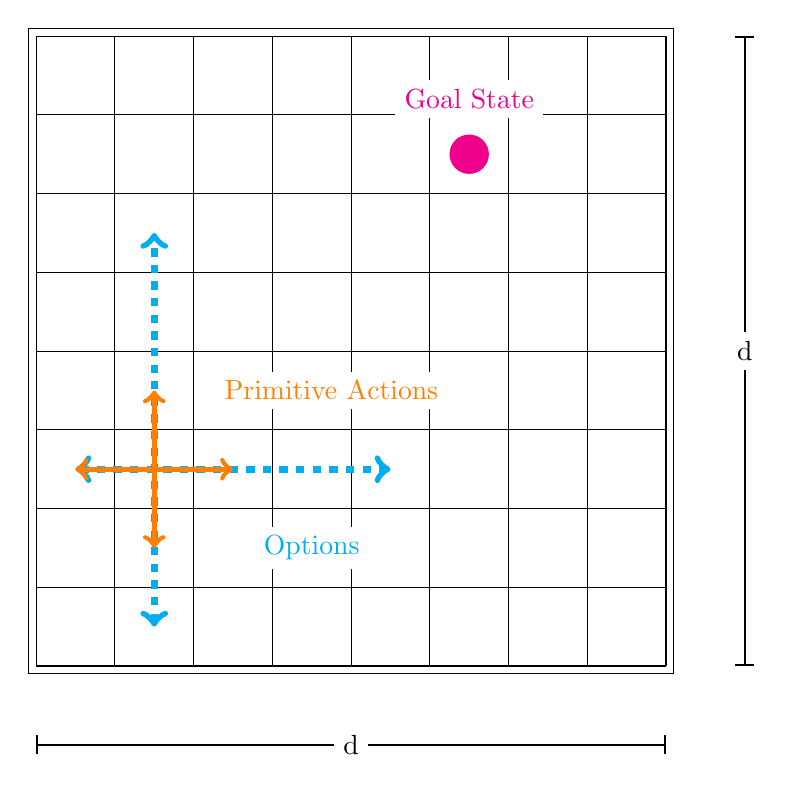
\begin{tikzpicture}
        \draw[step=1cm, color=black] (0,0) grid (8,8);
        \draw[black] (-0.1, -0.1) rectangle (8.1, 8.1);
        
        \fill[magenta] (5.5, 6.5) circle (0.25cm);
        \node [magenta, fill=white] at (5.5, 7.2) {Goal State};
        
        \draw [<->, line width=0.85mm, cyan, dashed] (1.5, 0.5) -- (1.5, 5.5);
        \draw [<->, line width=0.85mm, cyan, dashed] (0.5, 2.5) -- (4.5, 2.5);
        
        \draw [<->, line width=0.65mm, orange] (1.5, 1.5) -- (1.5, 3.5);
        \draw [<->, line width=0.65mm, orange] (0.5, 2.5) -- (2.5, 2.5);
        
        \node [orange, fill=white] at (3.75, 3.5) {Primitive Actions};
        \node [cyan, fill=white] at (3.5, 1.5) {Options};
        
        \draw [|-|, line width=0.25mm] (9, 0) -- (9, 8) node [midway, fill=white] {d};
        \draw [|-|, line width=0.25mm] (0, -1) -- (8, -1) node [midway, fill=white] {d};
    \end{tikzpicture}
    
    \caption{Grid-world domain}
    \label{fig:grid_domain}
\end{figure}

When the goal state is reached, the agent is teleported to any of the $d^2$ states with uniform probability.
The agent receives a reward of $r_{max}$ when it transitions from the goal state to any other state; for all other state transitions, it receives 0 reward.

At each state except the goal state 4 options are available, they are \texttt{UP}, \texttt{DOWN}, \texttt{LEFT} and \texttt{RIGHT}.
Each option terminates after a maximum of $m$ steps. 
In other words, when an option, say \texttt{UP} is chosen, it executes the primitive action \texttt{UP} at most $m$ time and then terminates.
A state $s^\prime$ that is $k$ steps away from the starting state $s$ and $n$ steps away from the nearest boundary wall along the direction of the movement of the option has a probability of termination $\beta_o(s^\prime) = 1/(\min\{m, n\} - k + 1)$ where $k \in [\min\{m, n\}]$.
Thus, the maximum holding time for any option can be at most be $m$ units.

In the goal state, there is a single option available that terminates after one step, providing a reward of $r_{max}$ to the learner and causing the agent to teleport to a random location on the grid with uniform probability.
The holding time for this special teleport option is a single time step.

The policy for each of the options $\pi_o$ at each of the states is stationary and is defined by the type of the option.
For example, the \texttt{UP} option only executes the \texttt{UP} action.

In our implementation, each of the states are number from 0 through $d^2 - 1$ starting from the top left corner and ending at the bottom right corner of the grid.


\section{Experiments and Results}

100 trials of learning in the grid world domain was executed for a time horizon of 200000 time steps.
During each trial the environment was randomly re-initialized such that the collected statistics were reset and both the agent as well as the goal state were moved to different locations on the grid.

The associated plots for accumulated regret and accumulated reward are shown in figures \ref{fig:regret} and  \ref{fig:reward}.
The gray error bands on the plot correspond to the 95\% confidence interval for the respective quantities being measured.

\begin{figure}[!htbp]
    \centering
    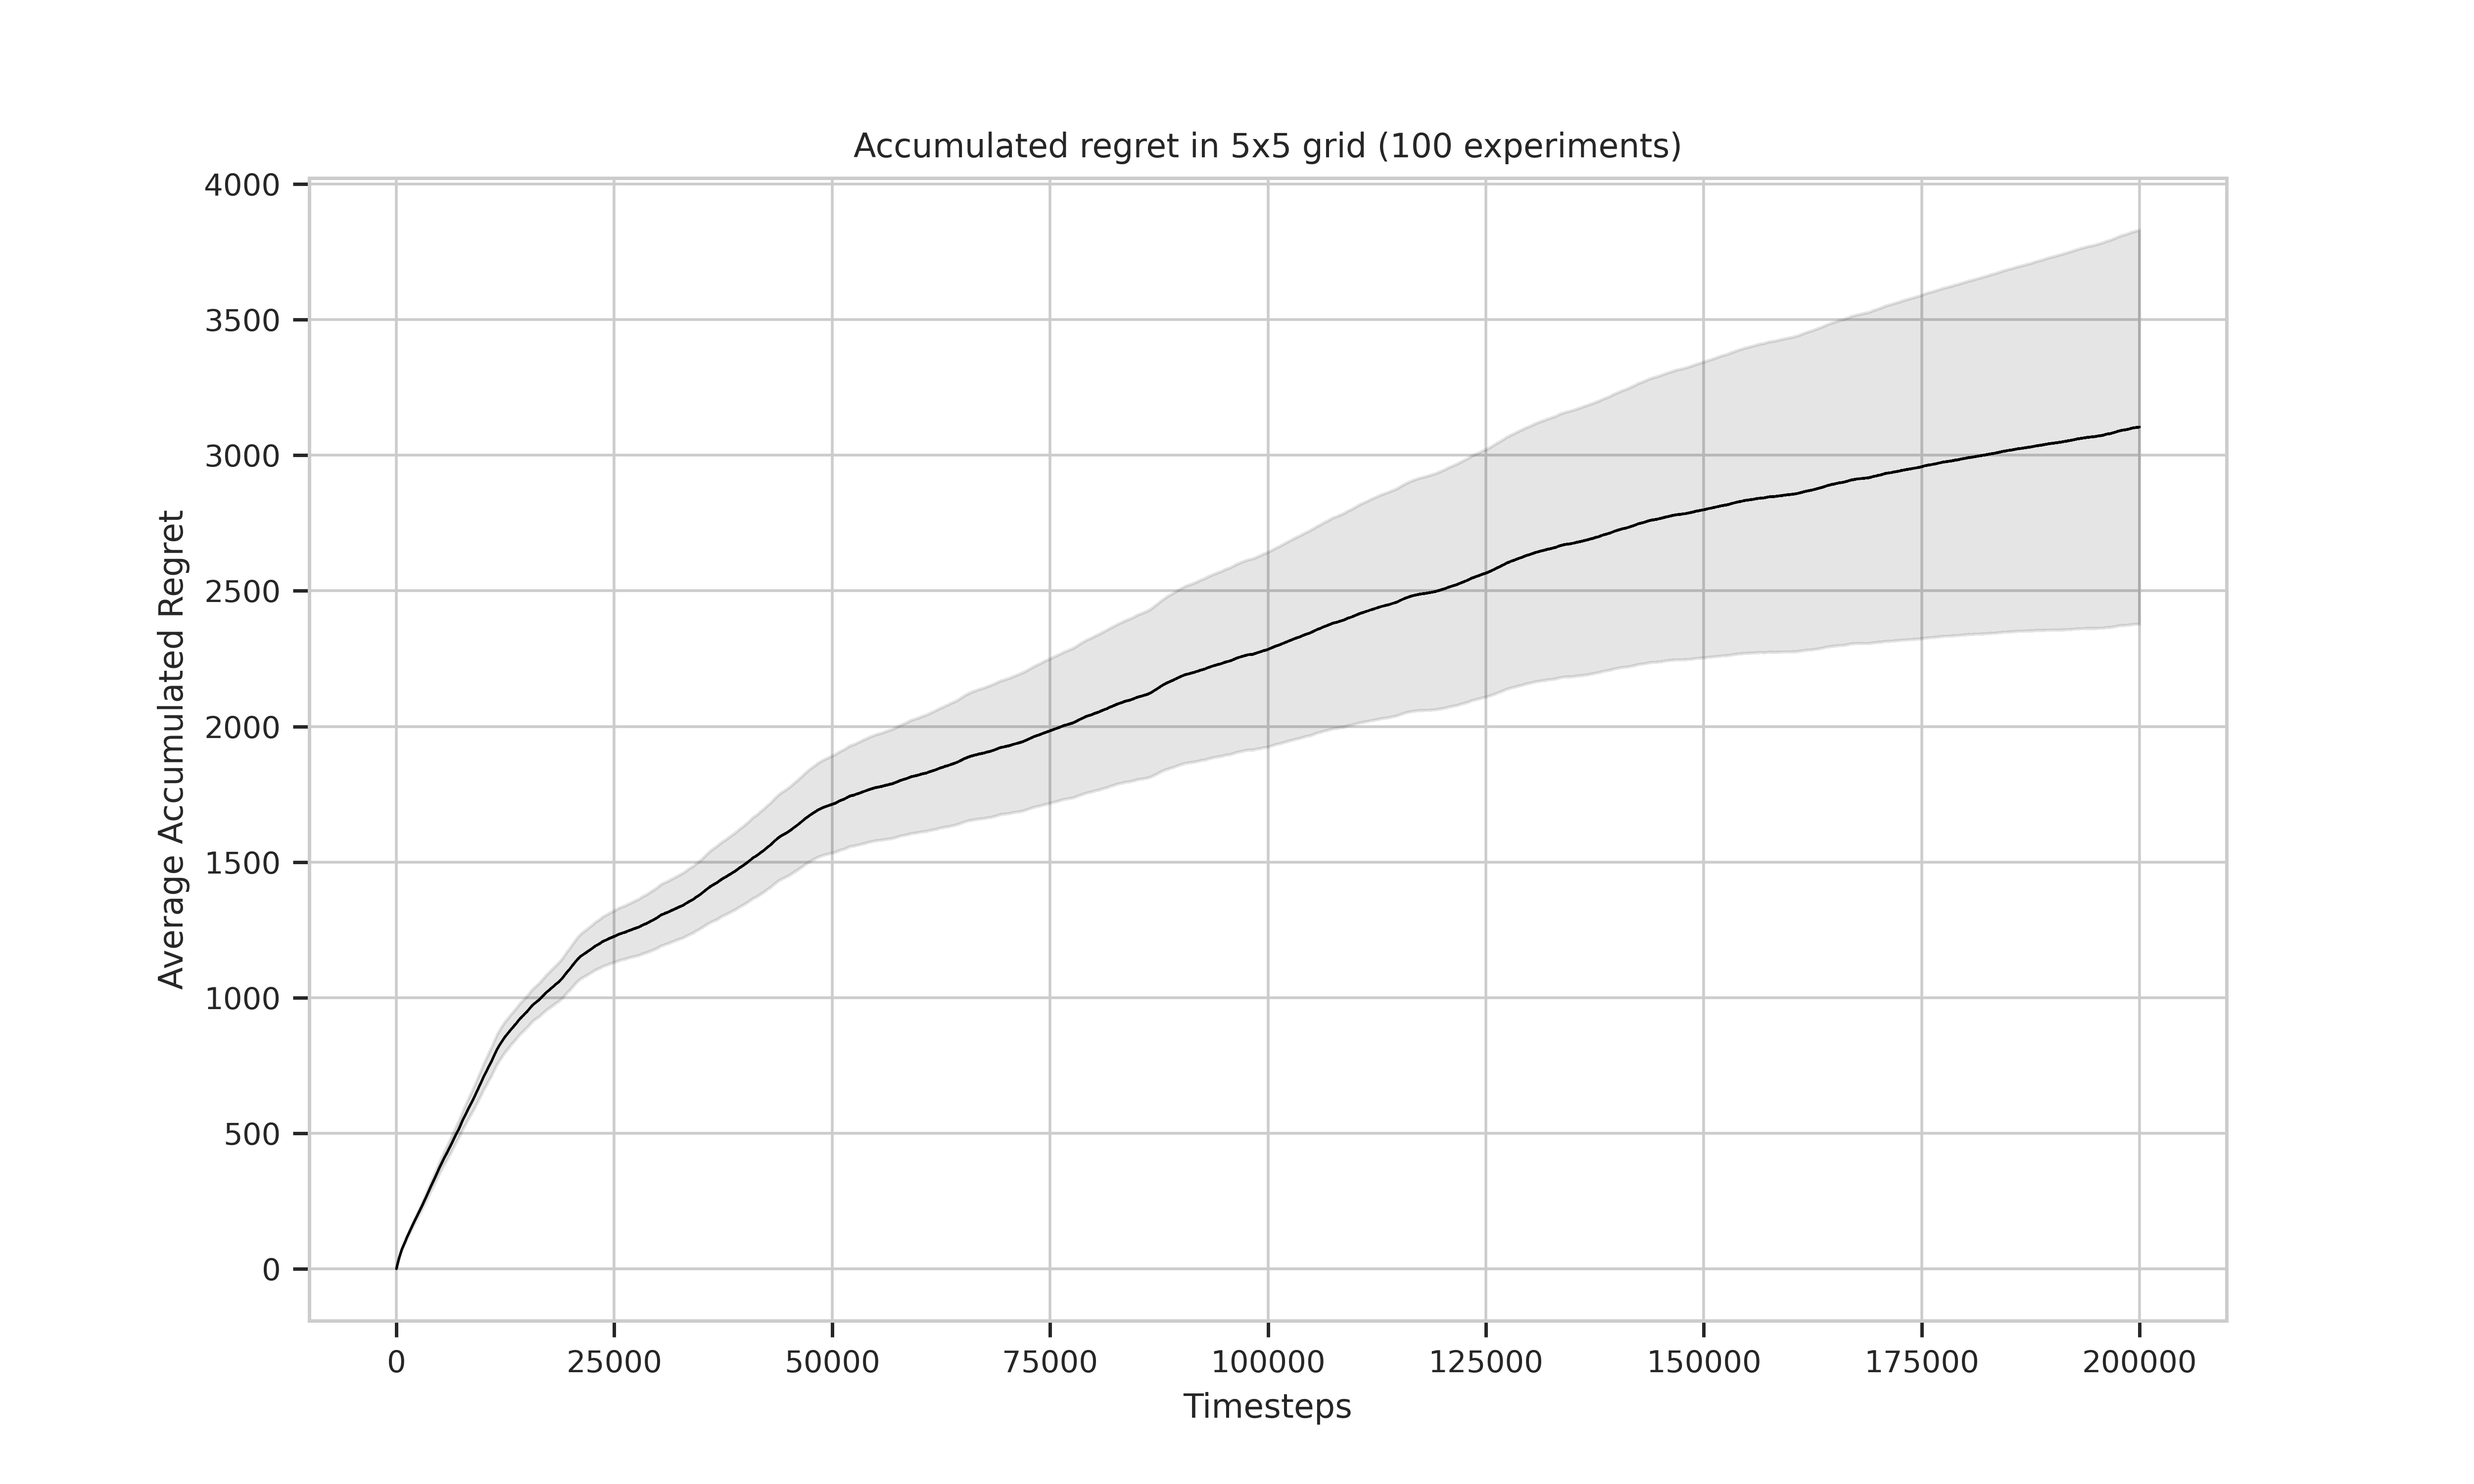
\includegraphics[width=\linewidth]{experimentation/images/Accumulated regret in 5x5 grid (100 experiments).png}
    \caption{Accumulated Regret for Grid World Domain}
    \label{fig:regret}
\end{figure}

It can be observed from figure \ref{fig:regret} that the accumulated regret follows a sub-linear trend.

\begin{figure}[!htbp]
    \centering
    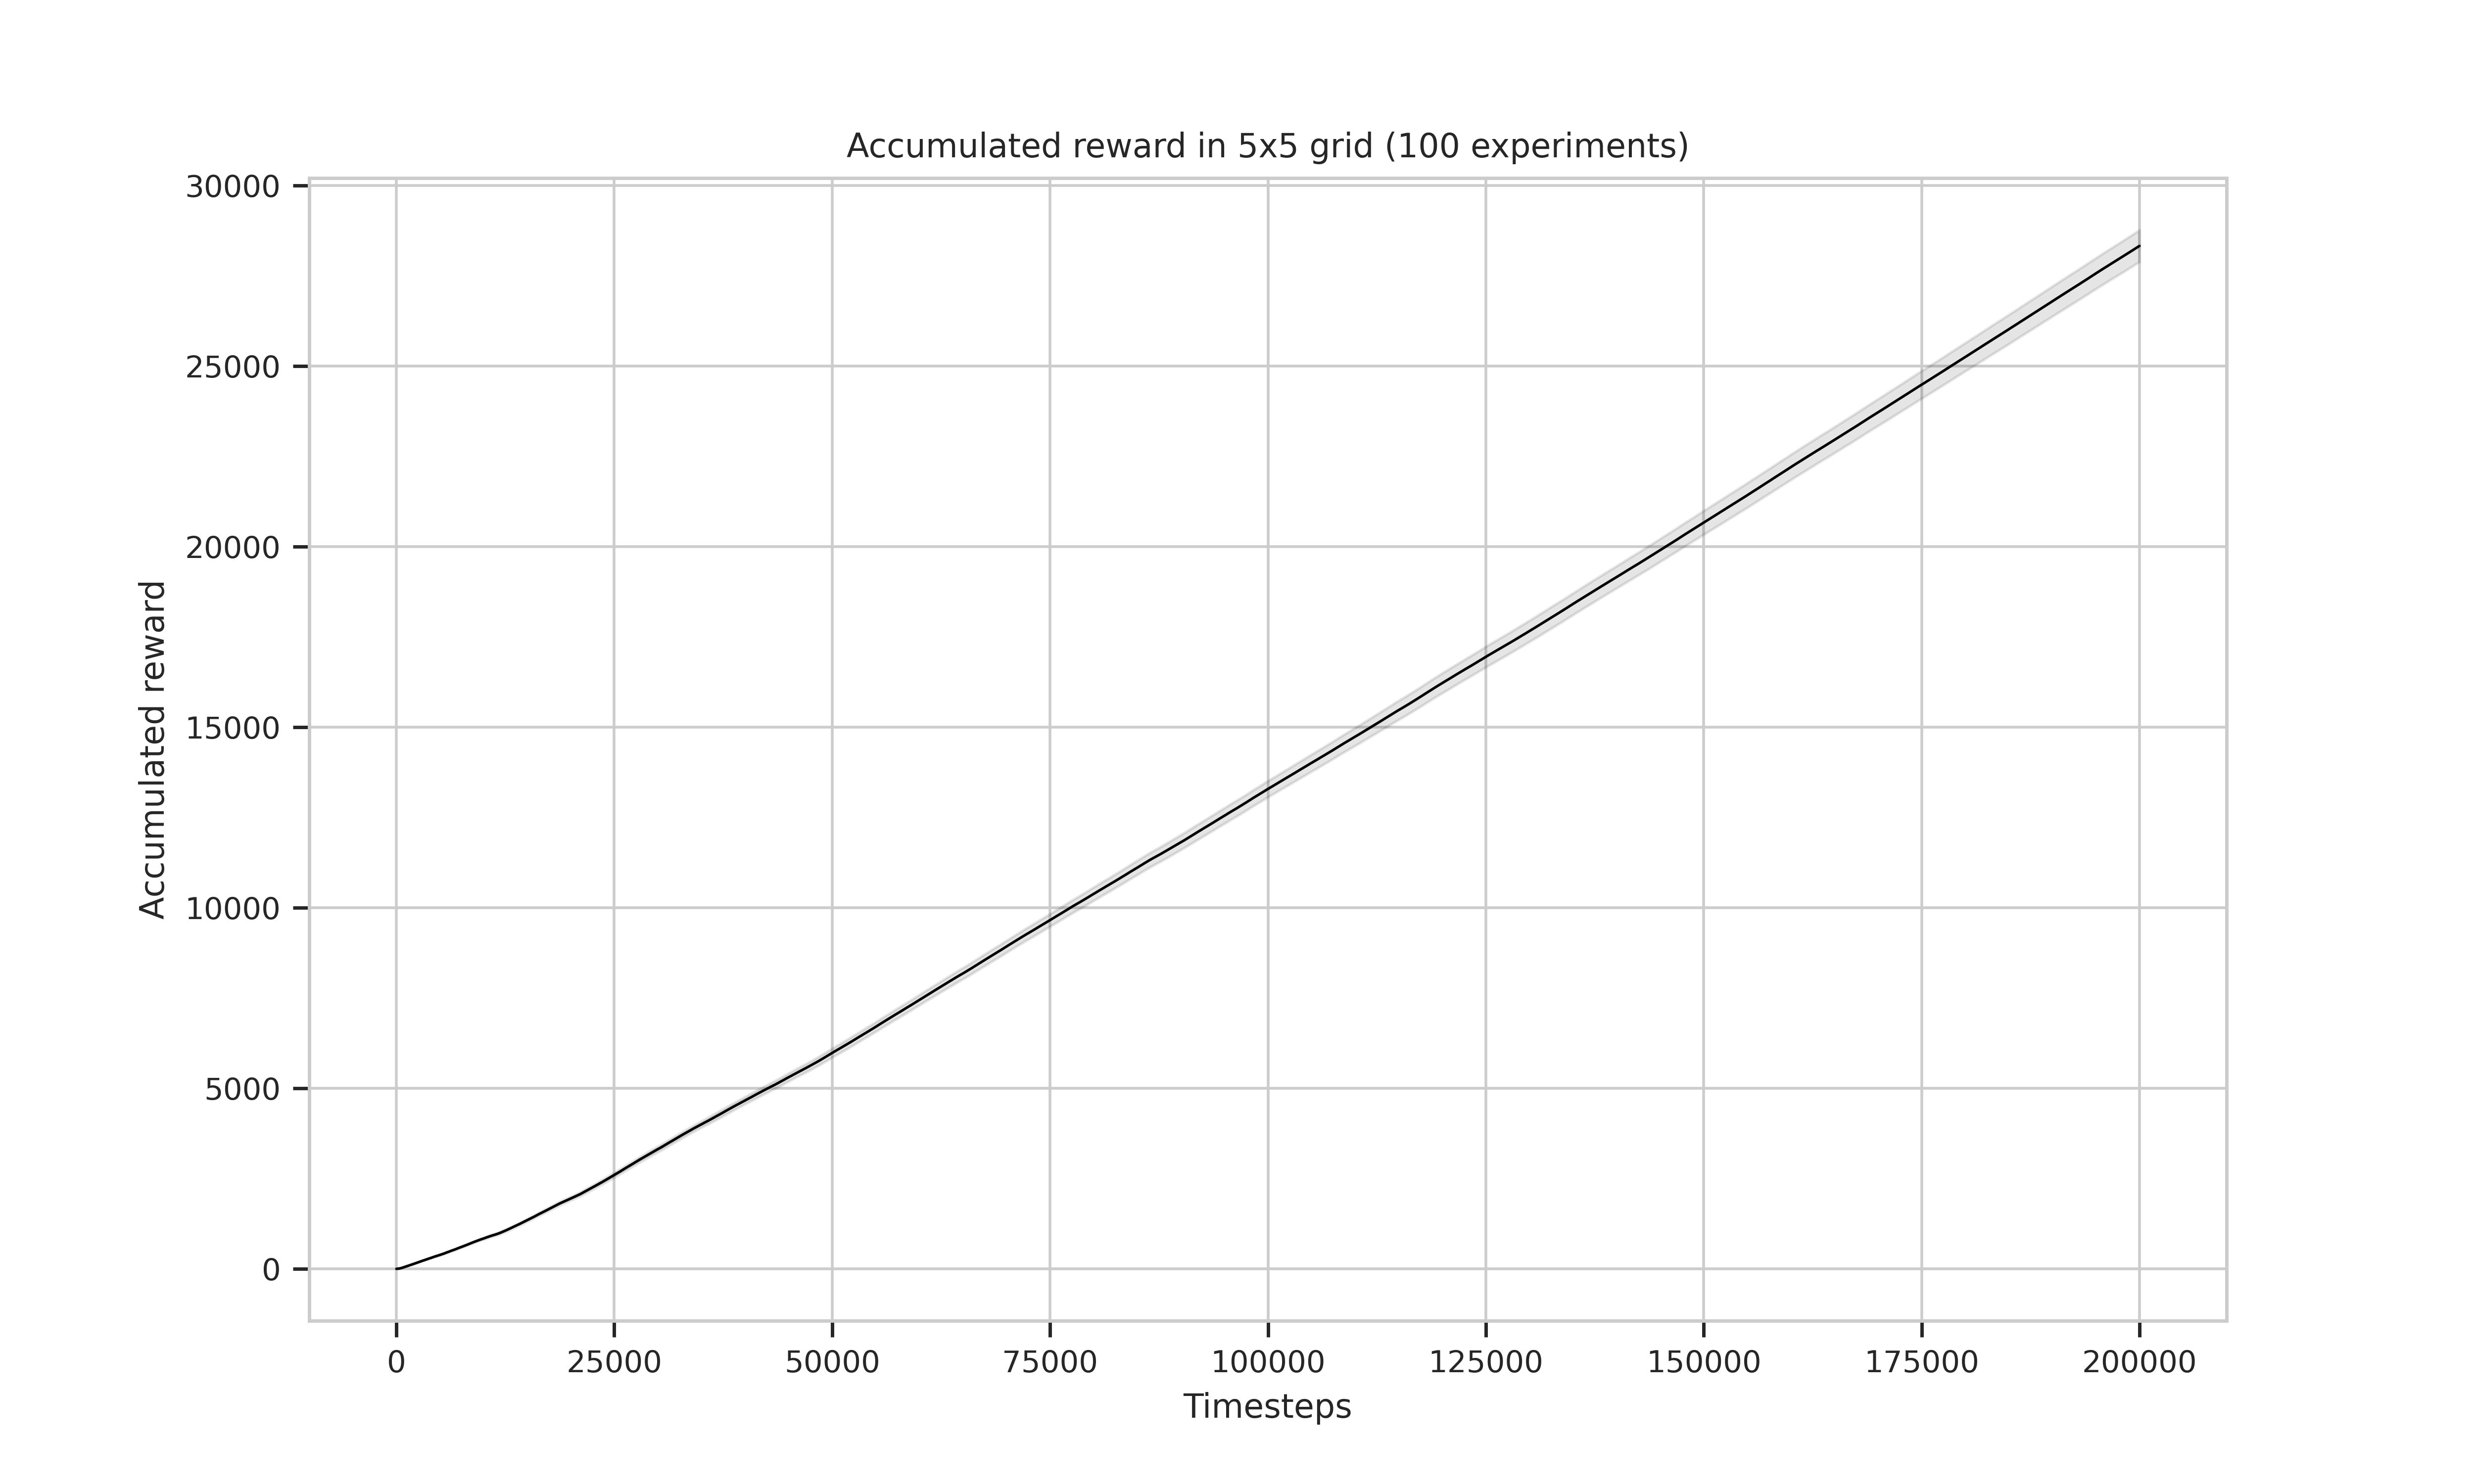
\includegraphics[width=\linewidth]{experimentation/images/Accumulated reward in 5x5 grid (100 experiments).png}
    \caption{Accumulated Reward for Grid World Domain}
    \label{fig:reward}
\end{figure}

It can also be observed from figure \ref{fig:reward} that the accumulated reward follows a linear trend.

The optimal policy as well as the learned policy are shown in figures \ref{fig:policy_1}, \ref{fig:policy_10}, \ref{fig:policy_12}, \ref{fig:policy_14} and \ref{fig:policy_20} for goal states 1, 10, 12, 14 and 20 in the grid world domain.

\begin{figure}[!htbp]
    \centering
    \begin{subfigure}[b]{0.49\linewidth}
        \centering
        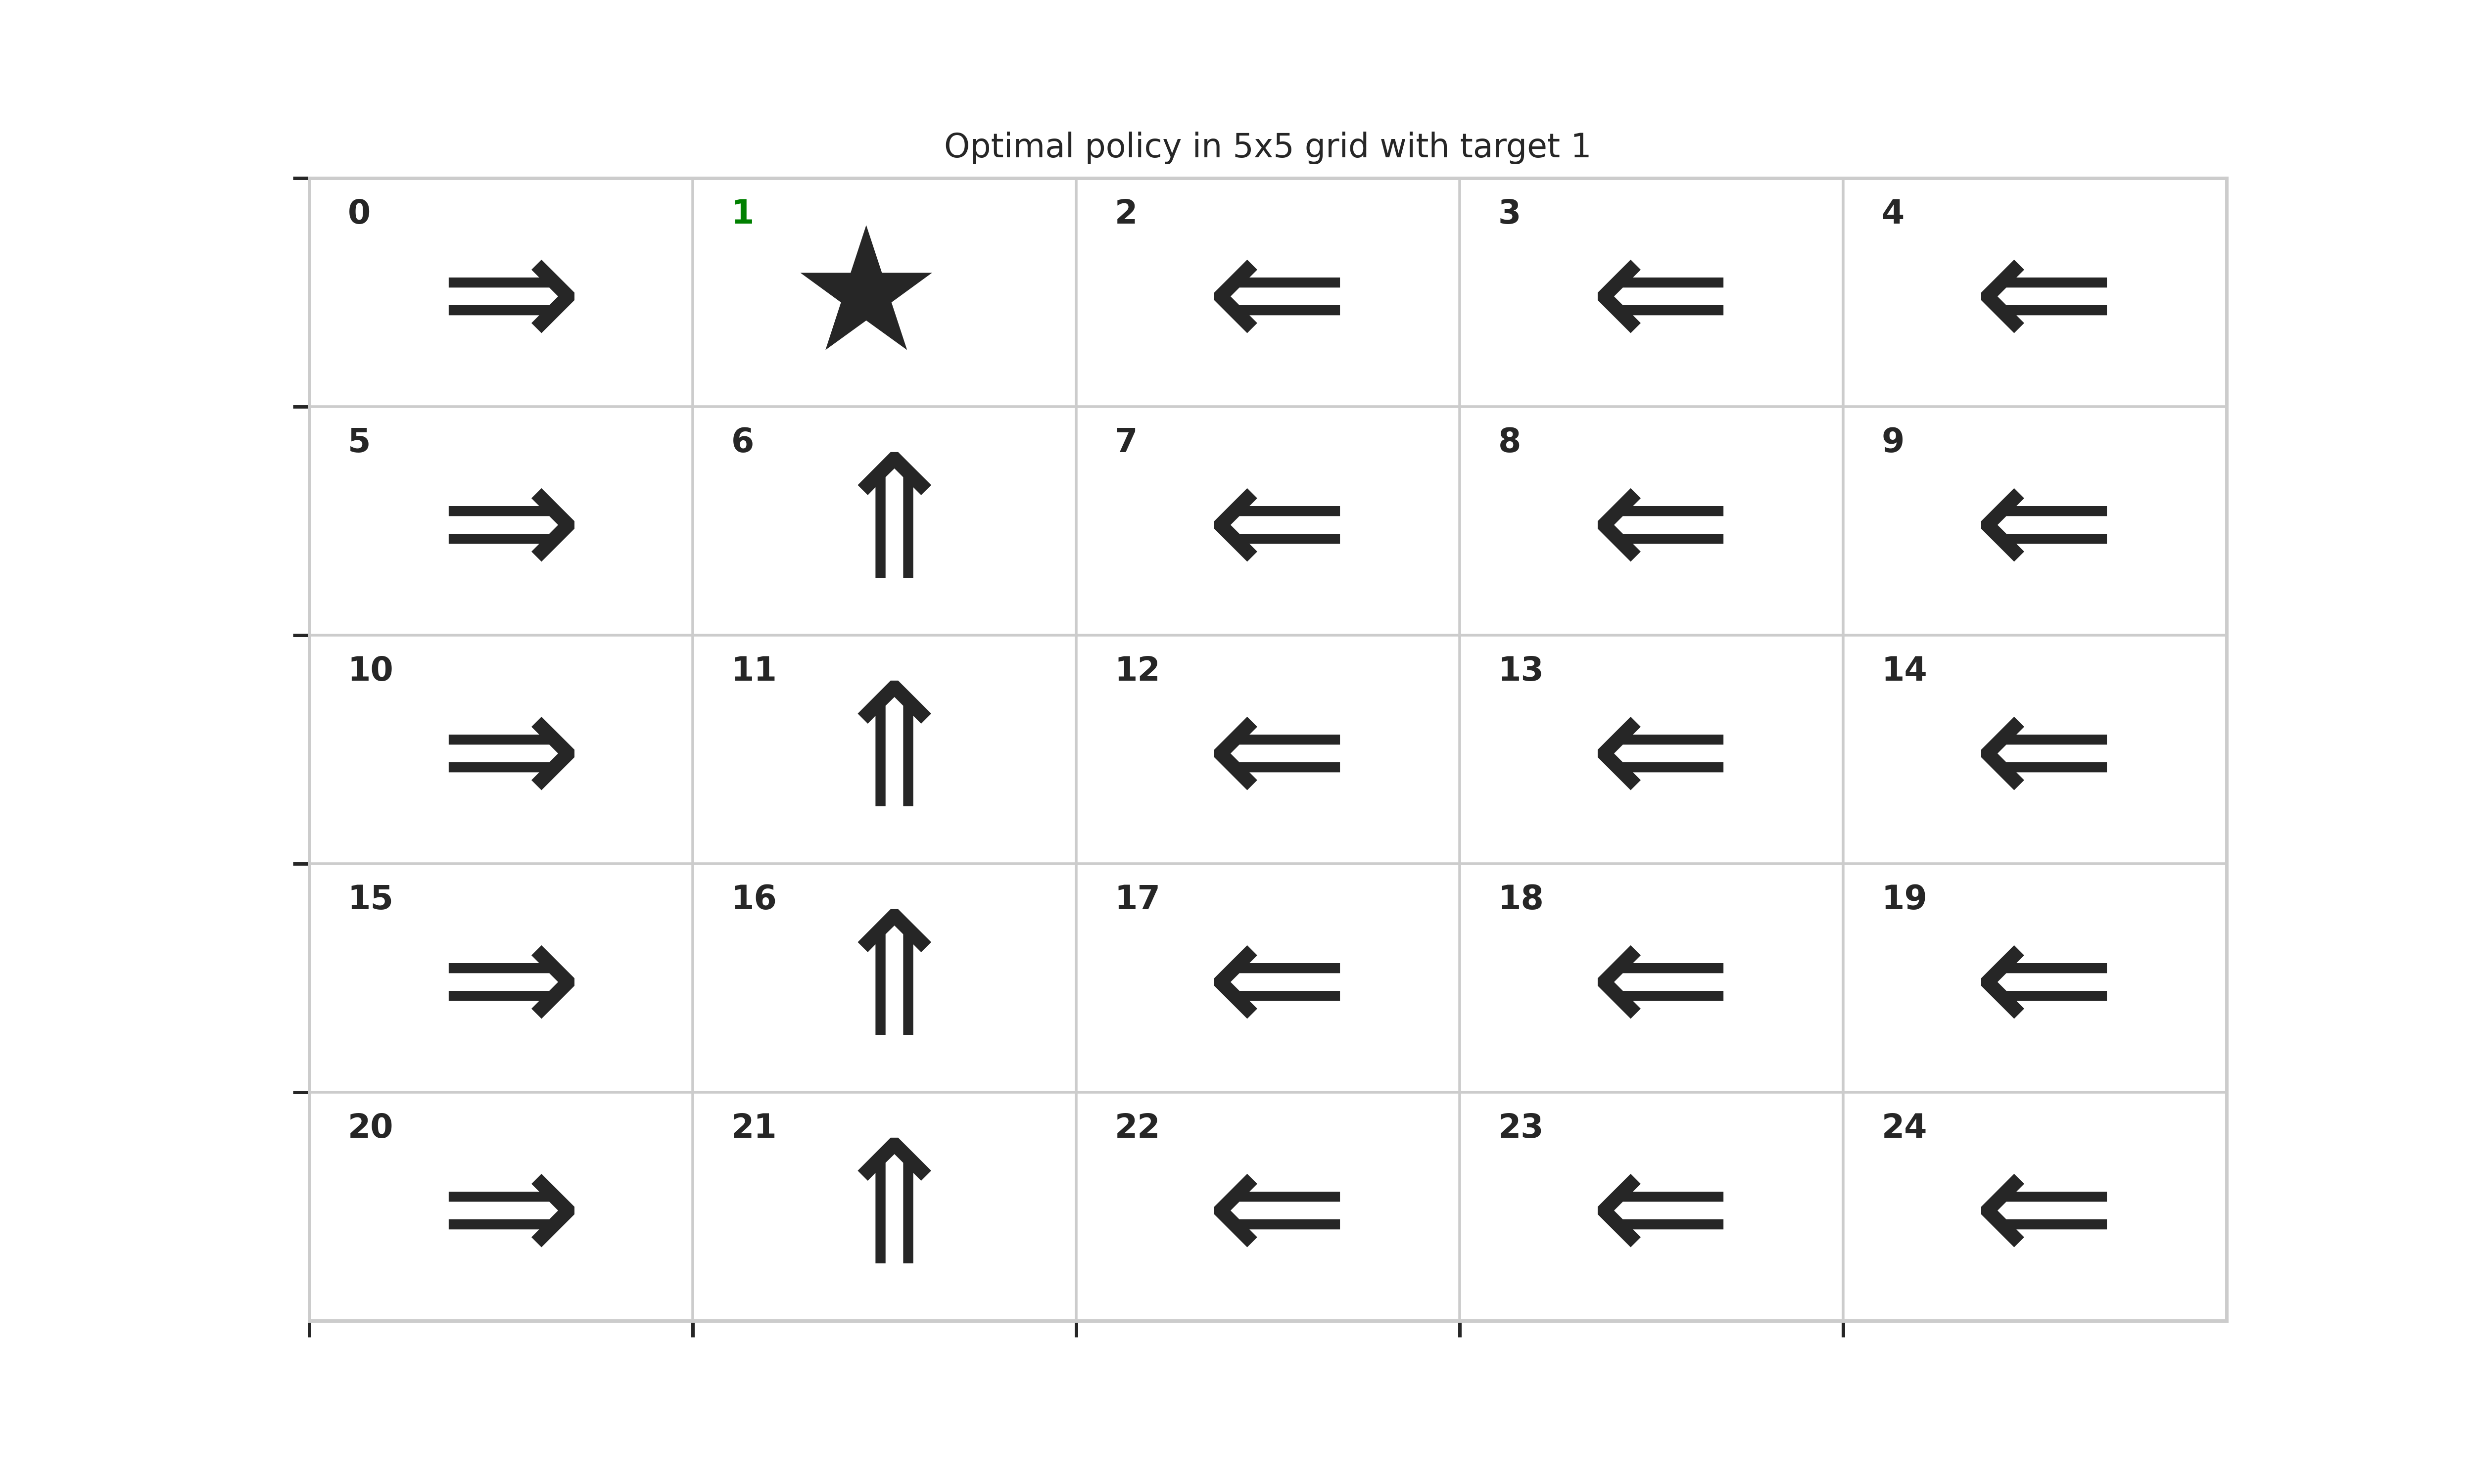
\includegraphics[width=\linewidth]{experimentation/images/Optimal policy in 5x5 grid with target 1.png}
        \caption{Optimal Policy}
    \end{subfigure}
    \begin{subfigure}[b]{0.49\linewidth}
        \centering
        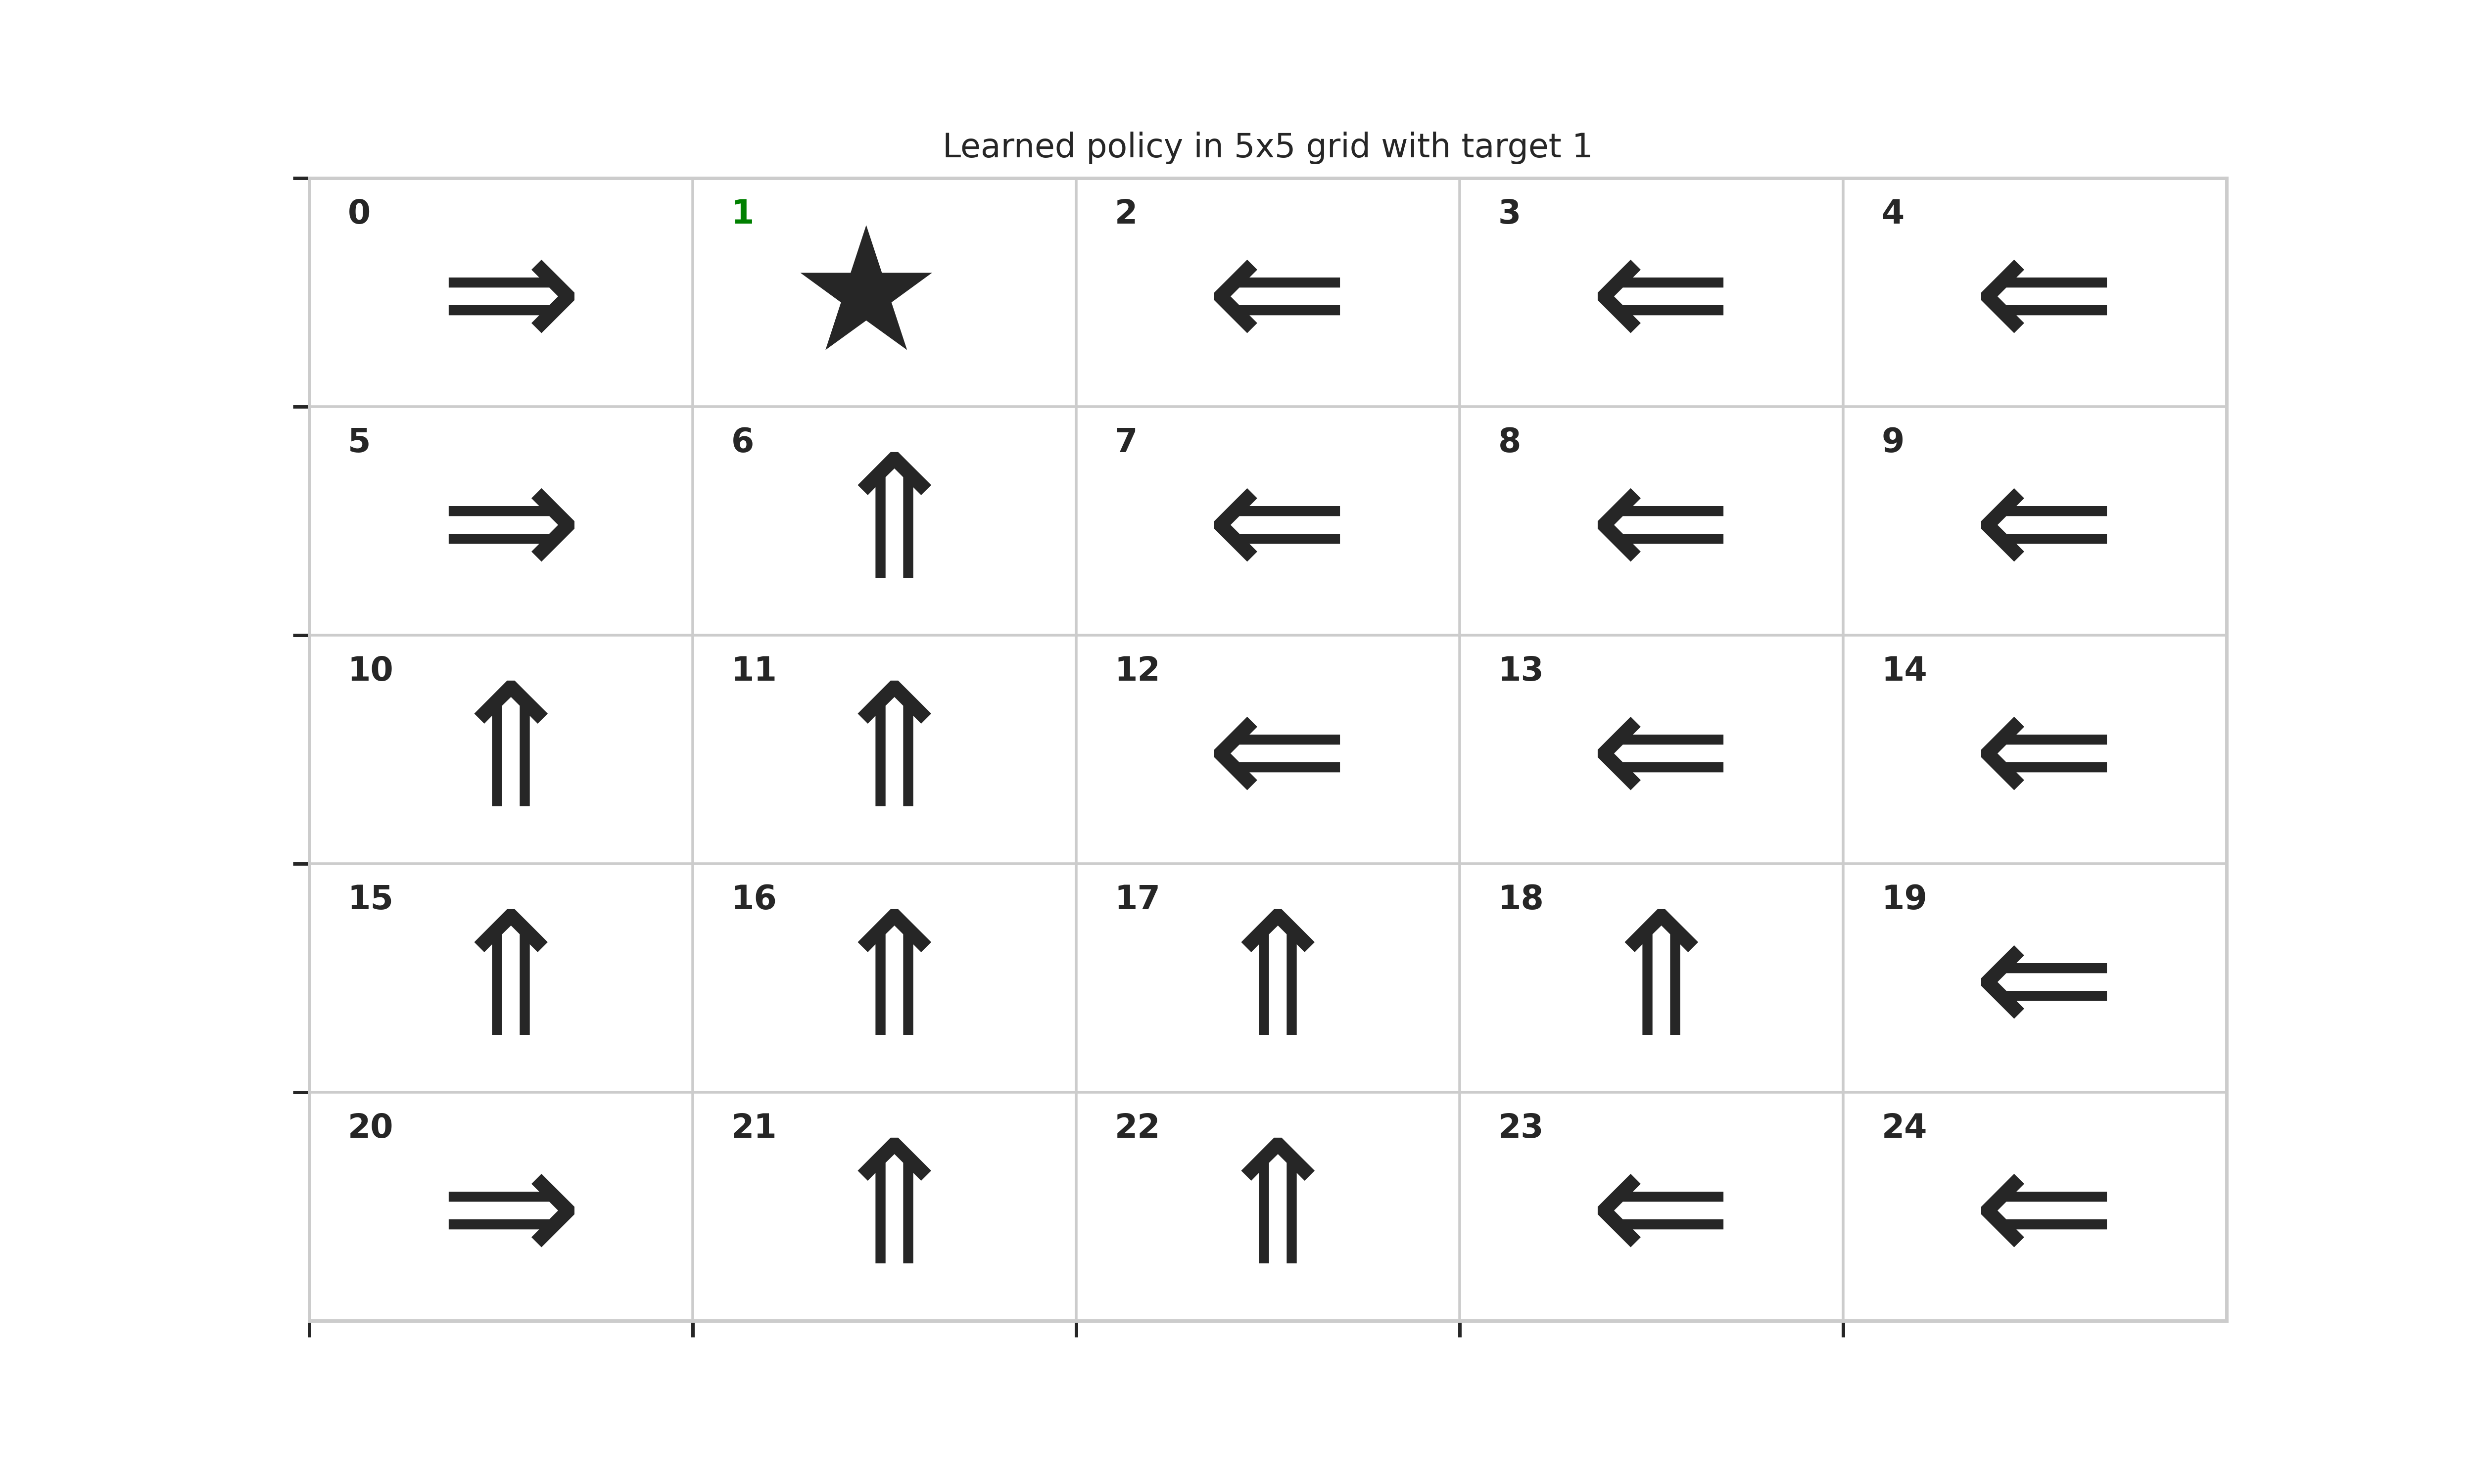
\includegraphics[width=\linewidth]{experimentation/images/Learned policy in 5x5 grid with target 1.png}
        \caption{Learned Policy}
    \end{subfigure}
    \caption{Policies for goal state set at 1.}
    \label{fig:policy_1}
\end{figure}

\begin{figure}[!htbp]
    \centering
    \begin{subfigure}[b]{0.49\linewidth}
        \centering
        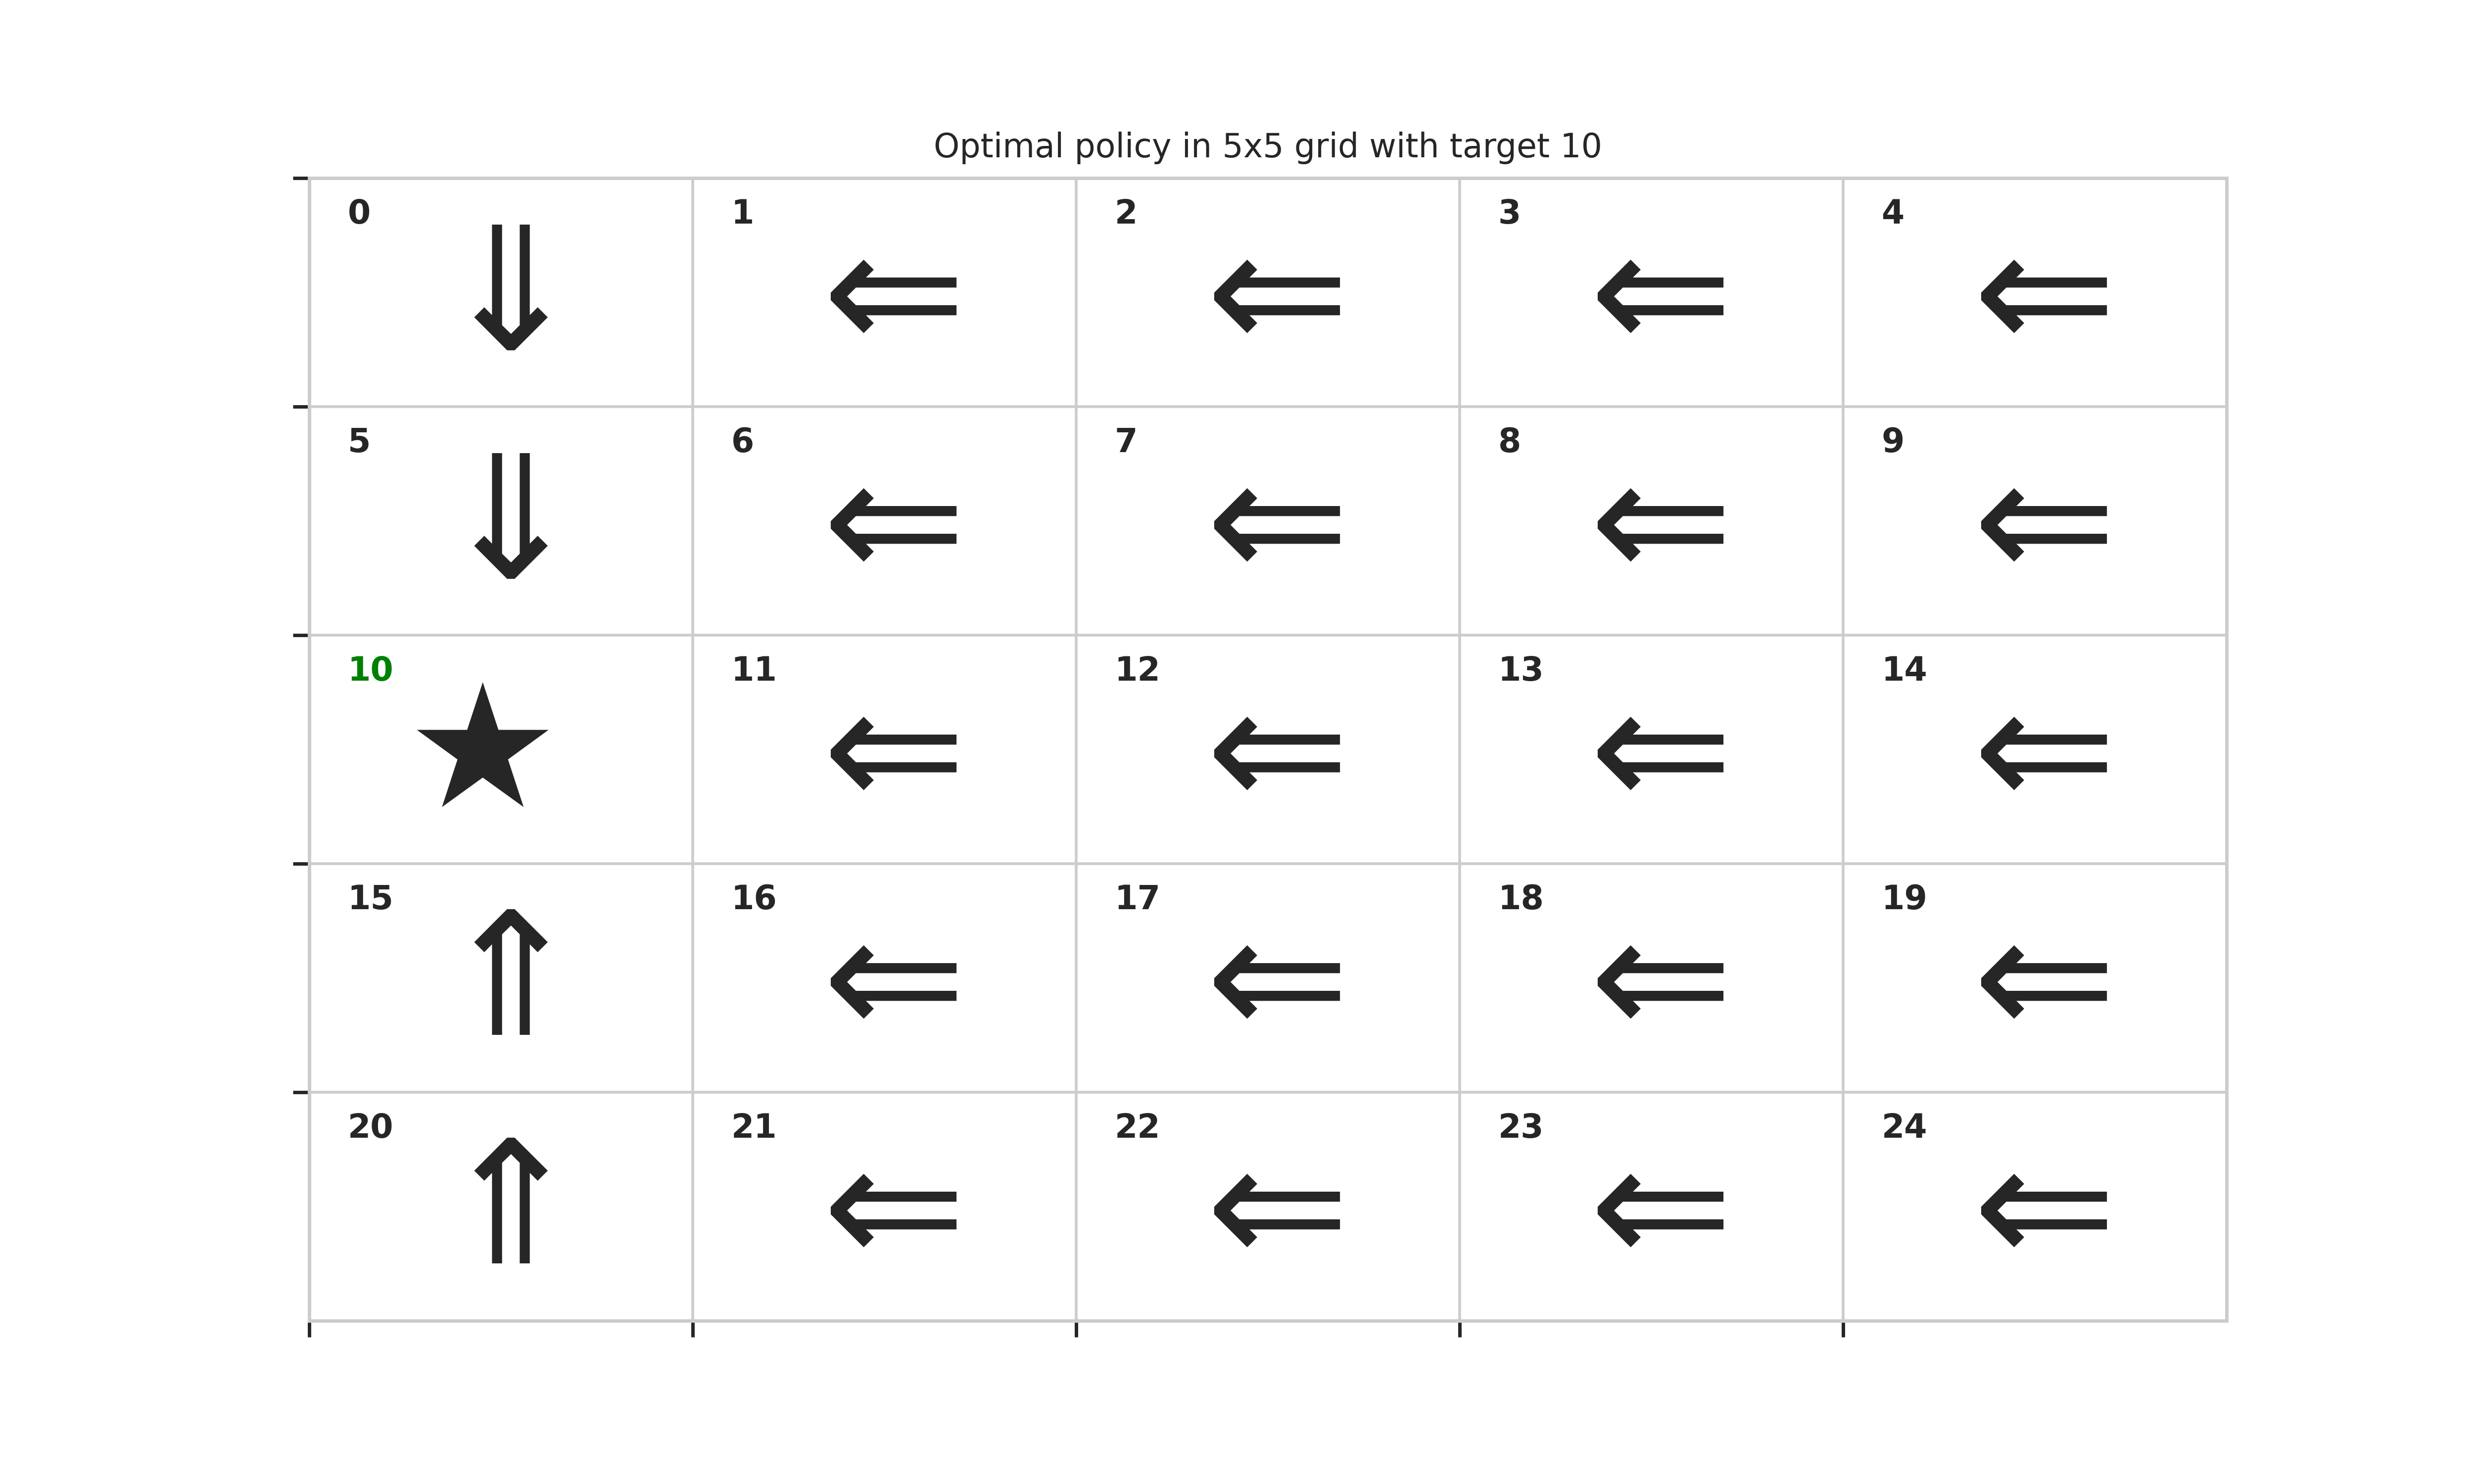
\includegraphics[width=\linewidth]{experimentation/images/Optimal policy in 5x5 grid with target 10.png}
        \caption{Optimal Policy}
    \end{subfigure}
    \begin{subfigure}[b]{0.49\linewidth}
        \centering
        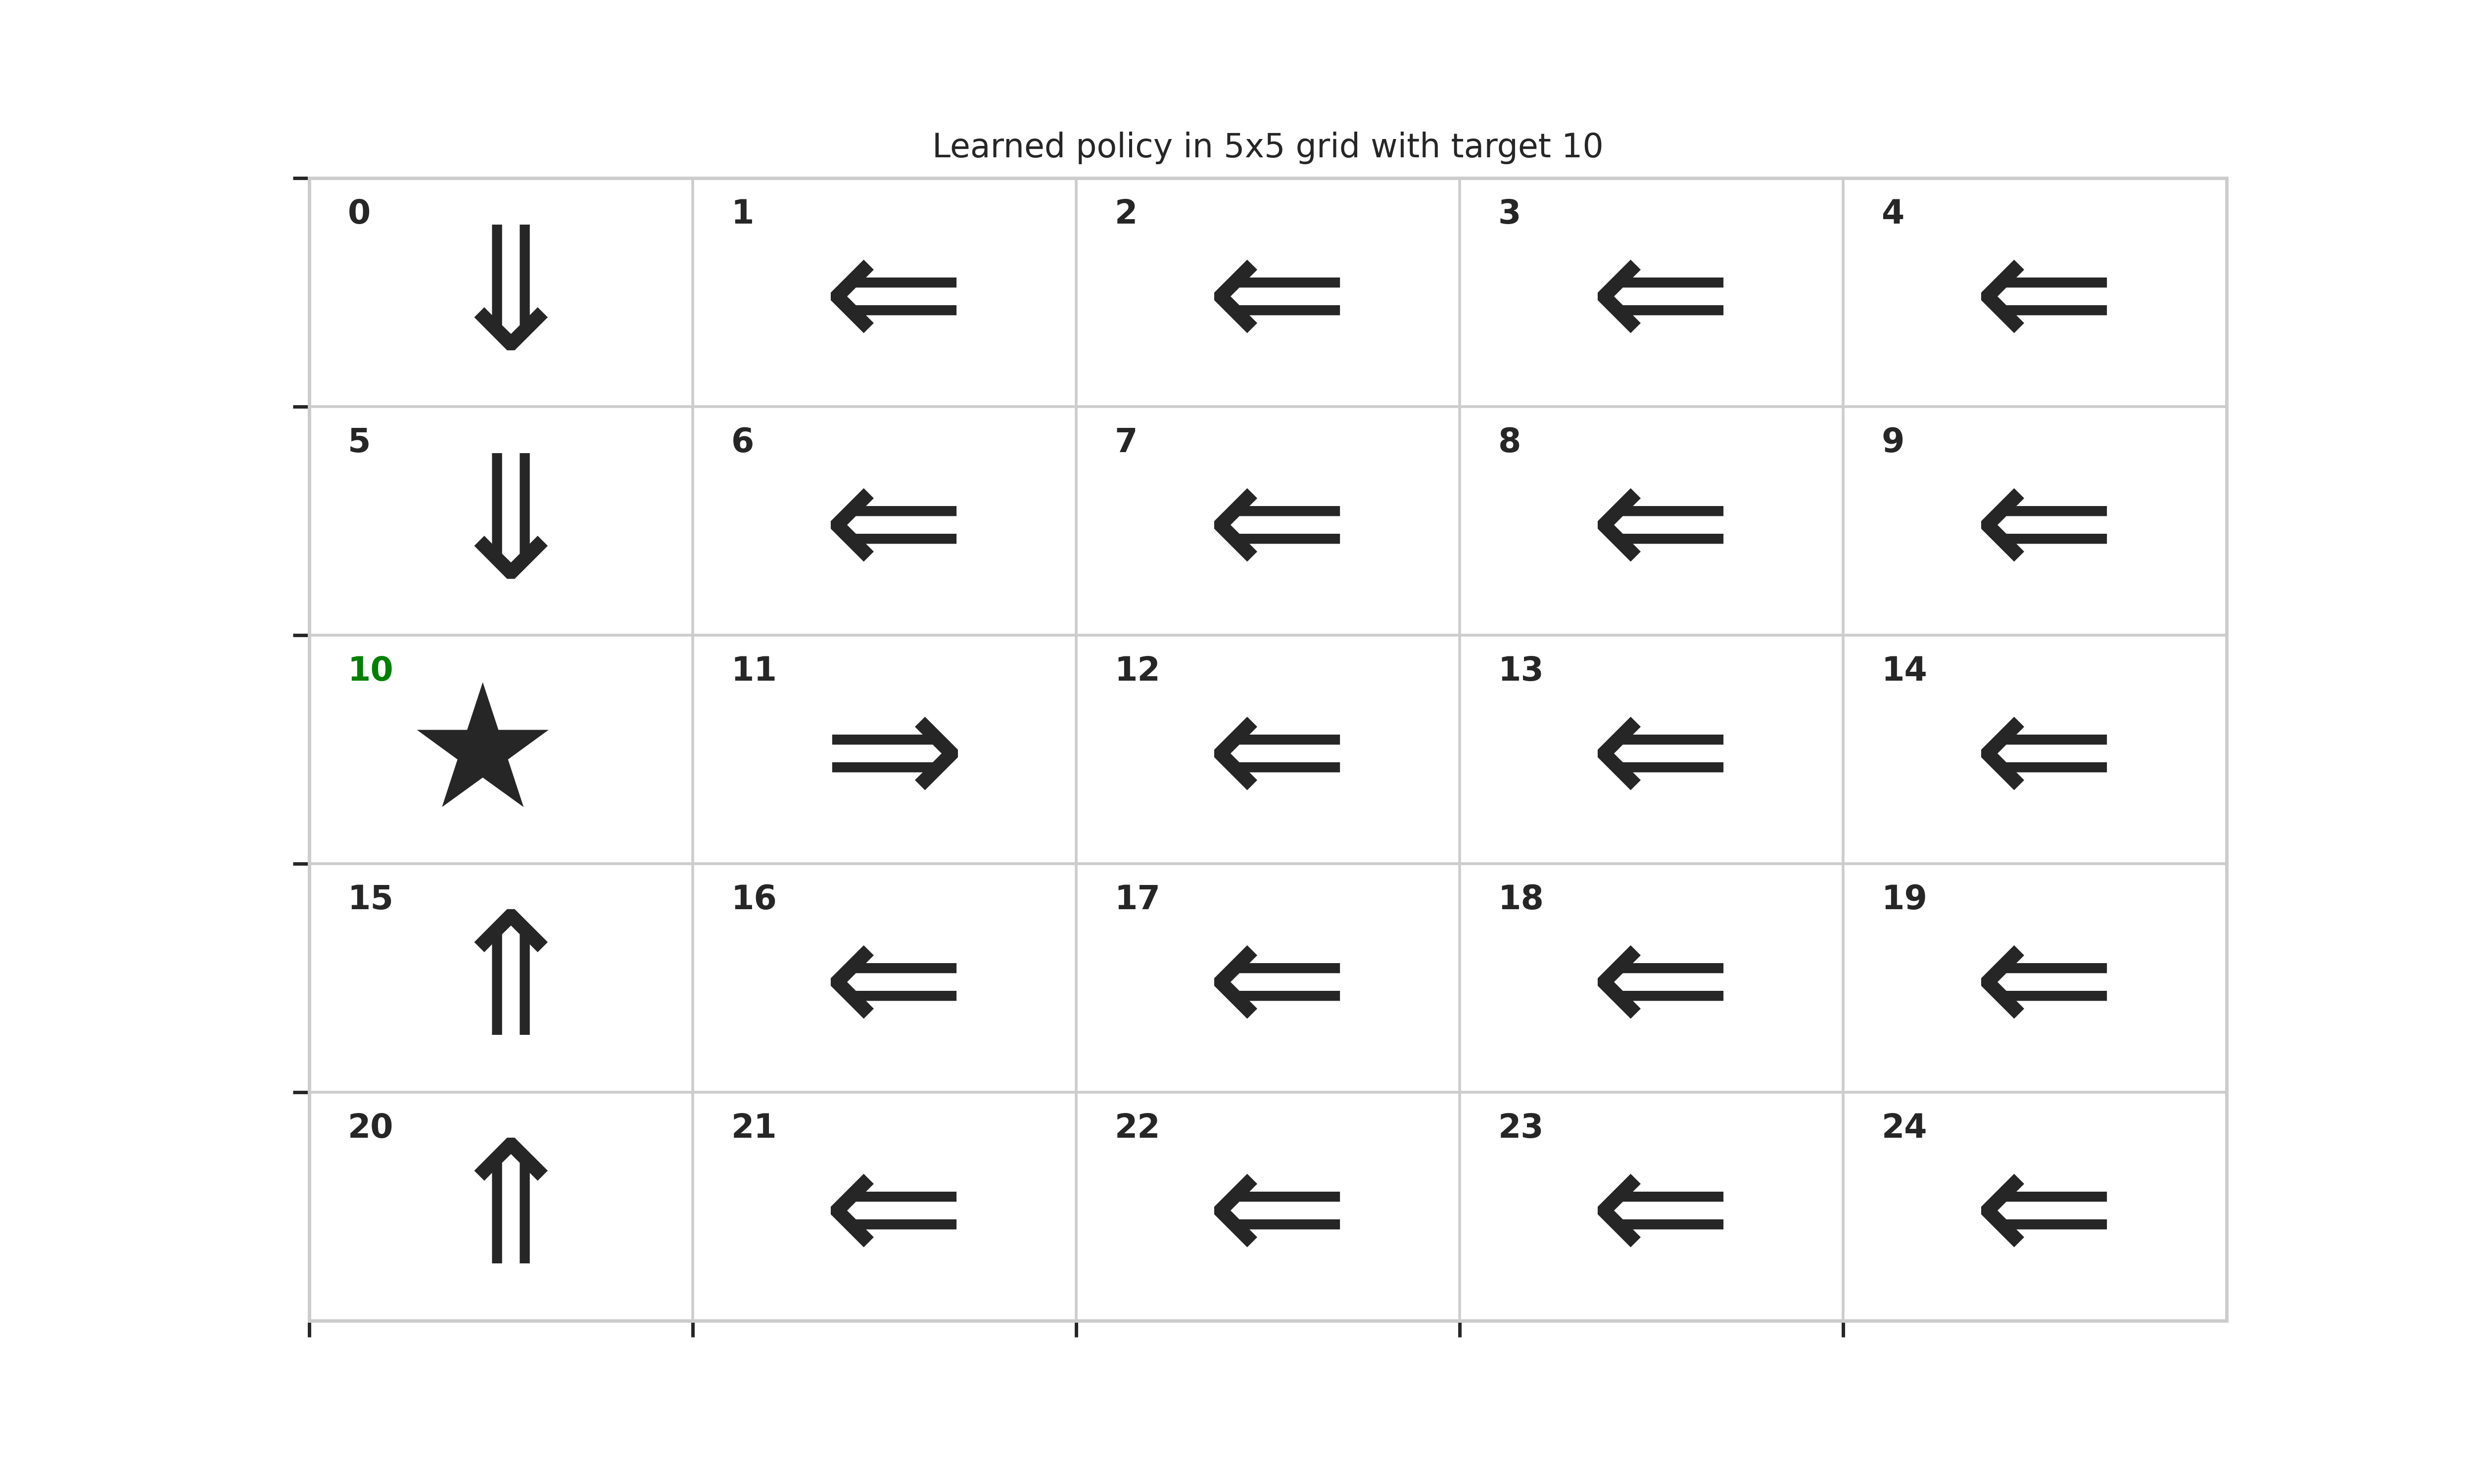
\includegraphics[width=\linewidth]{experimentation/images/Learned policy in 5x5 grid with target 10.png}
        \caption{Learned Policy}
    \end{subfigure}
    \caption{Policies for goal state set at 10.}
    \label{fig:policy_10}
\end{figure}

\begin{figure}[!htbp]
    \centering
    \begin{subfigure}[b]{0.49\linewidth}
        \centering
        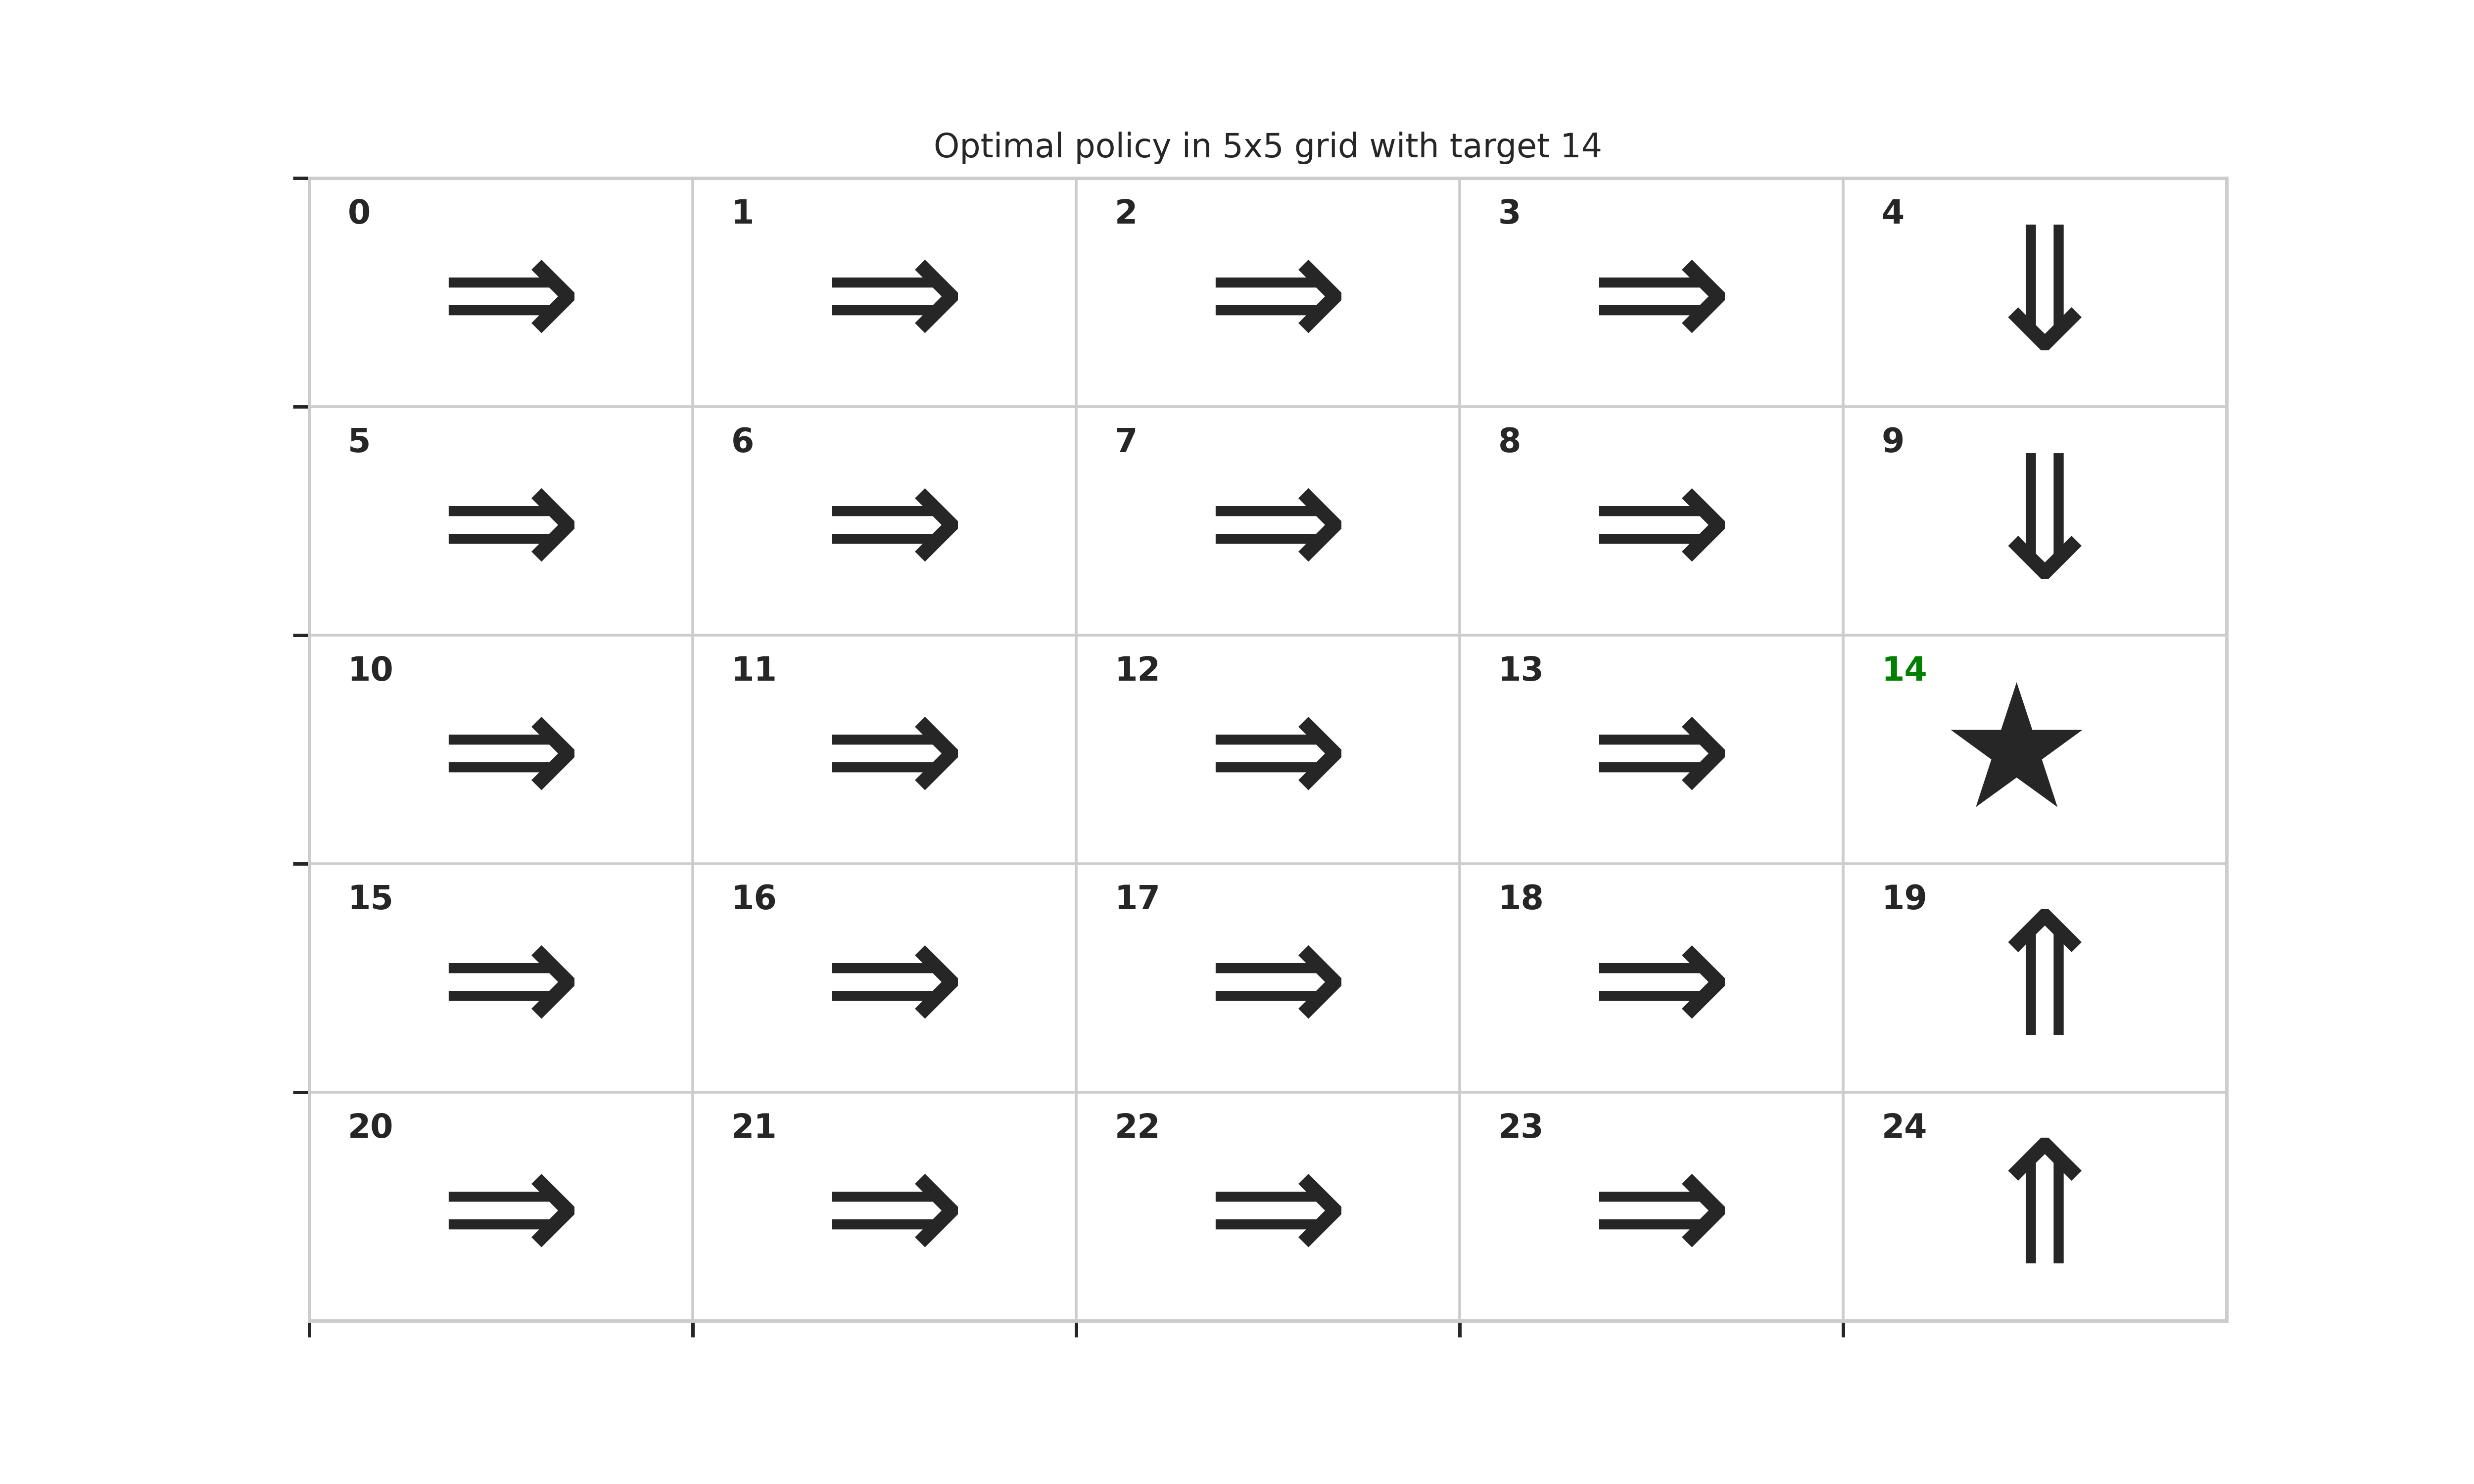
\includegraphics[width=\linewidth]{experimentation/images/Optimal policy in 5x5 grid with target 14.png}
        \caption{Optimal Policy}
    \end{subfigure}
    \begin{subfigure}[b]{0.49\linewidth}
        \centering
        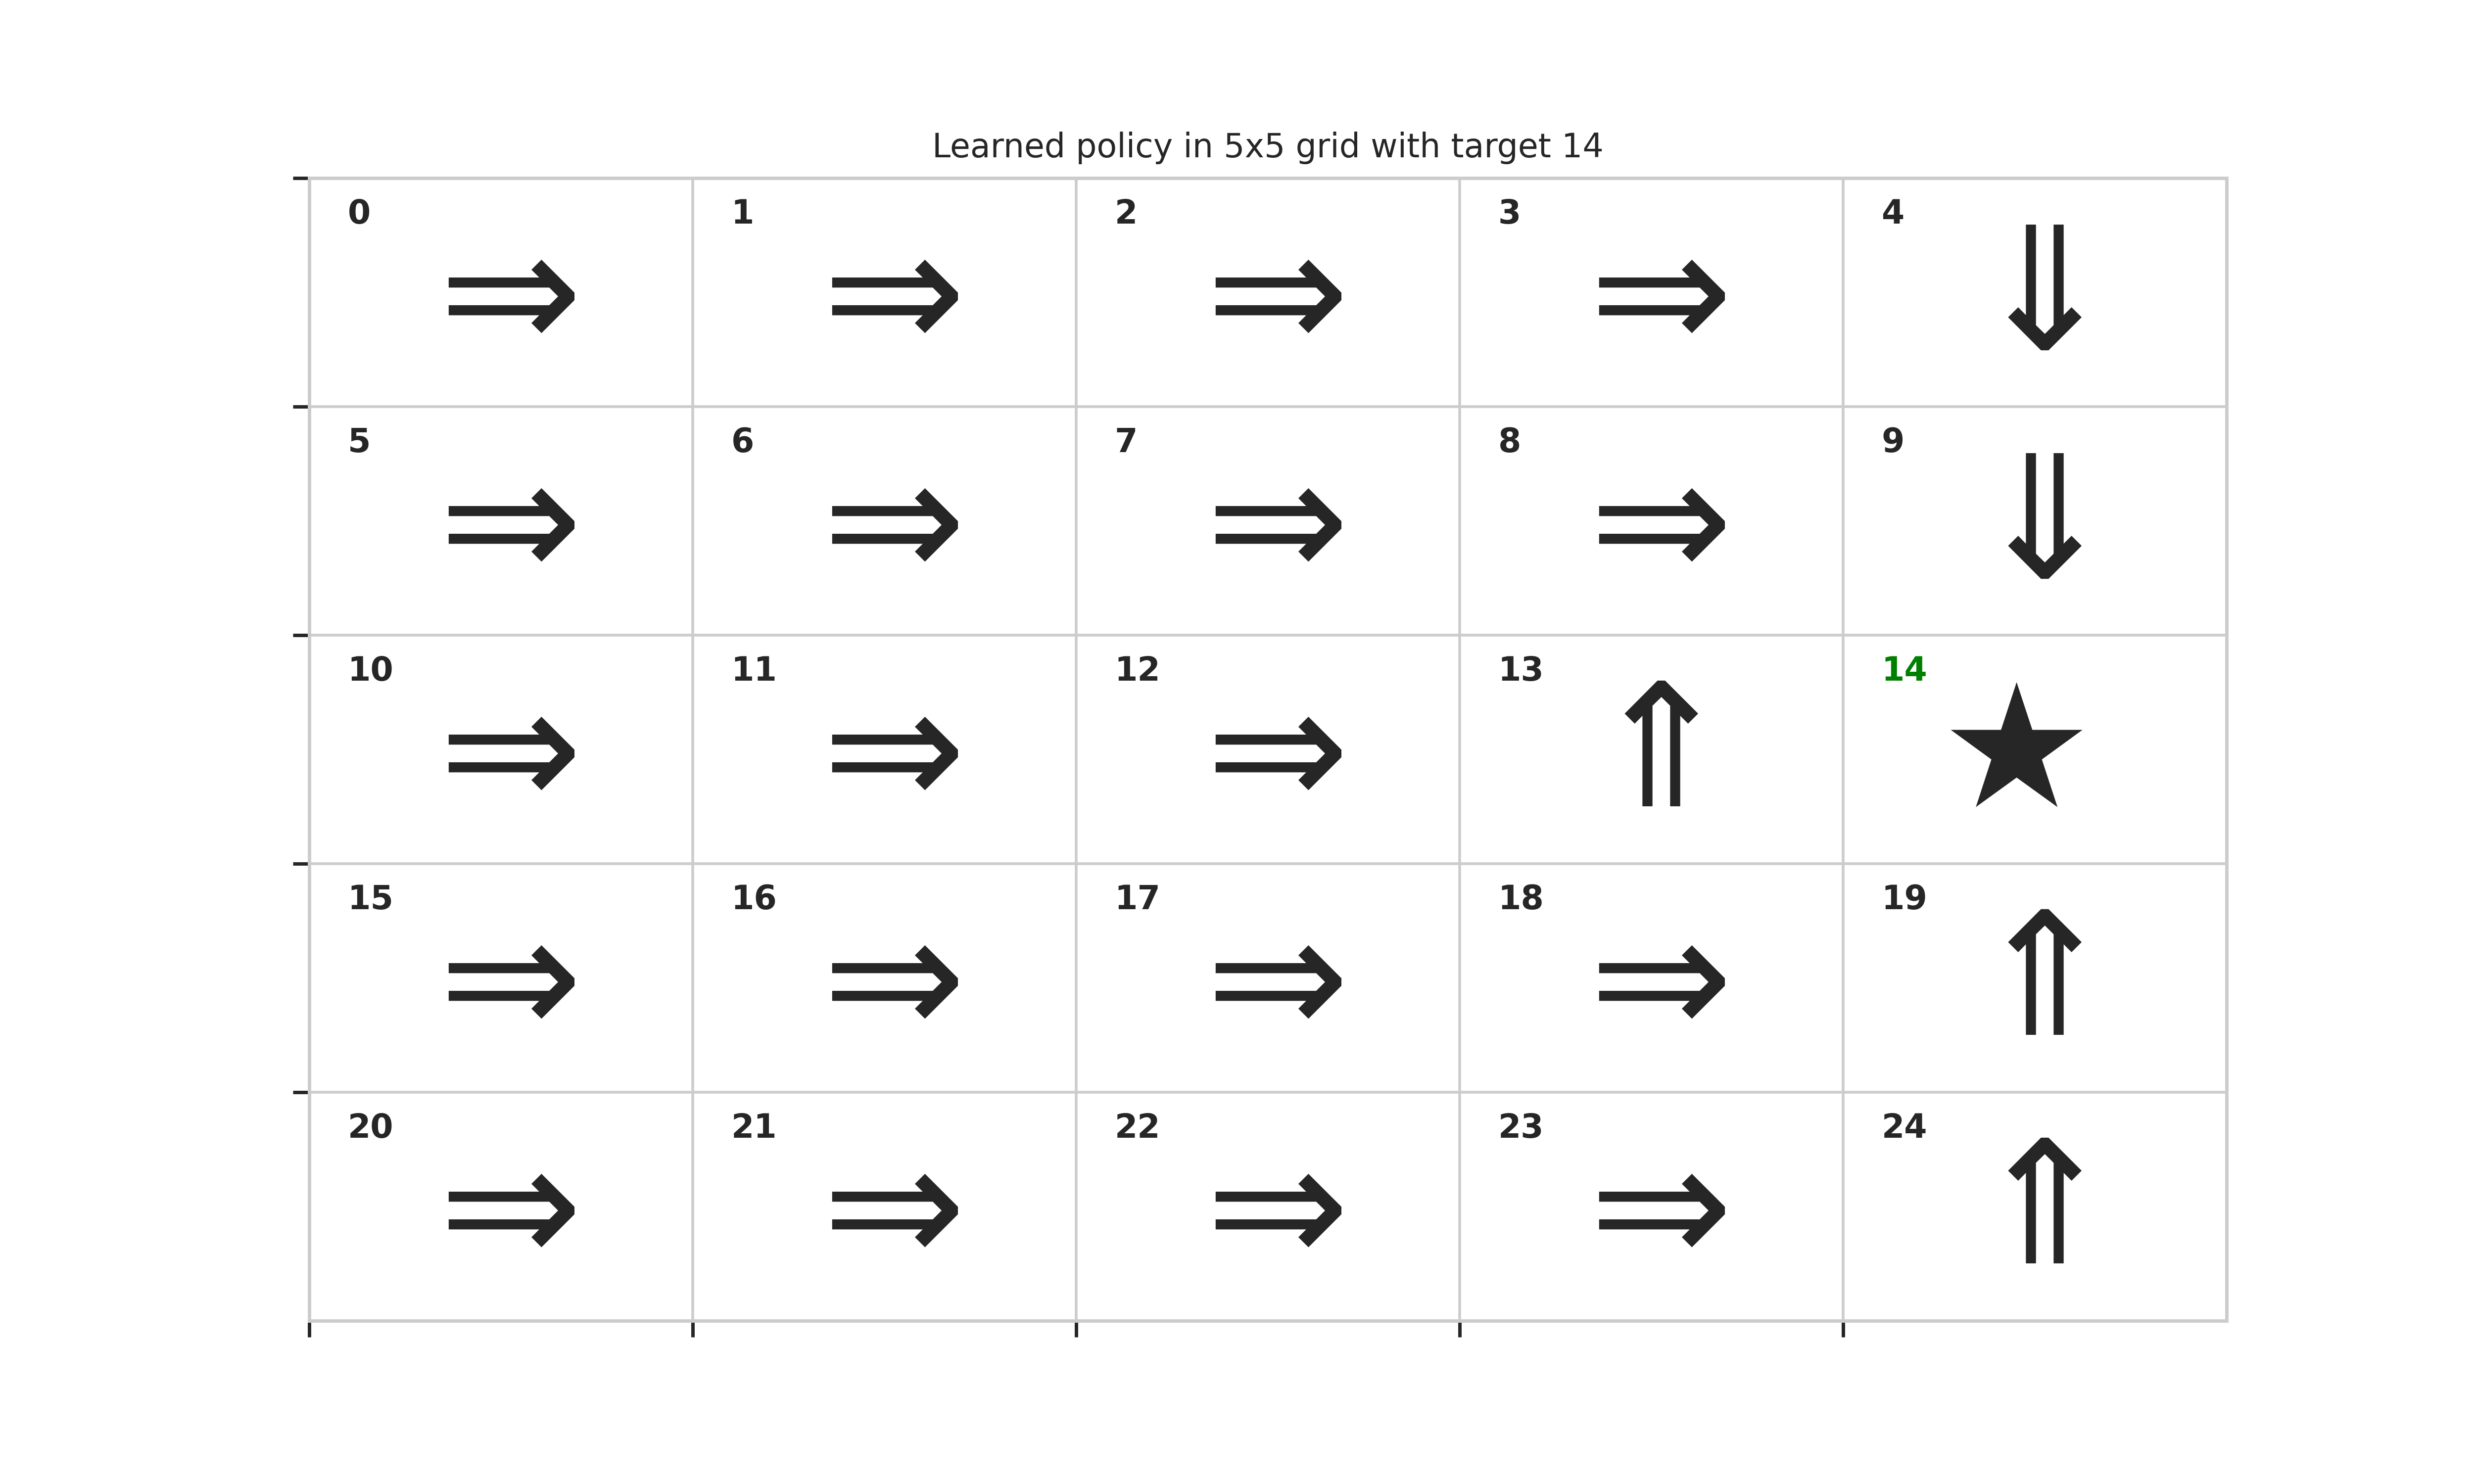
\includegraphics[width=\linewidth]{experimentation/images/Learned policy in 5x5 grid with target 14.png}
        \caption{Learned Policy}
    \end{subfigure}
    \caption{Policies for goal state set at 14.}
    \label{fig:policy_14}
\end{figure}

\begin{figure}[!htbp]
    \centering
    \begin{subfigure}[b]{0.49\linewidth}
        \centering
        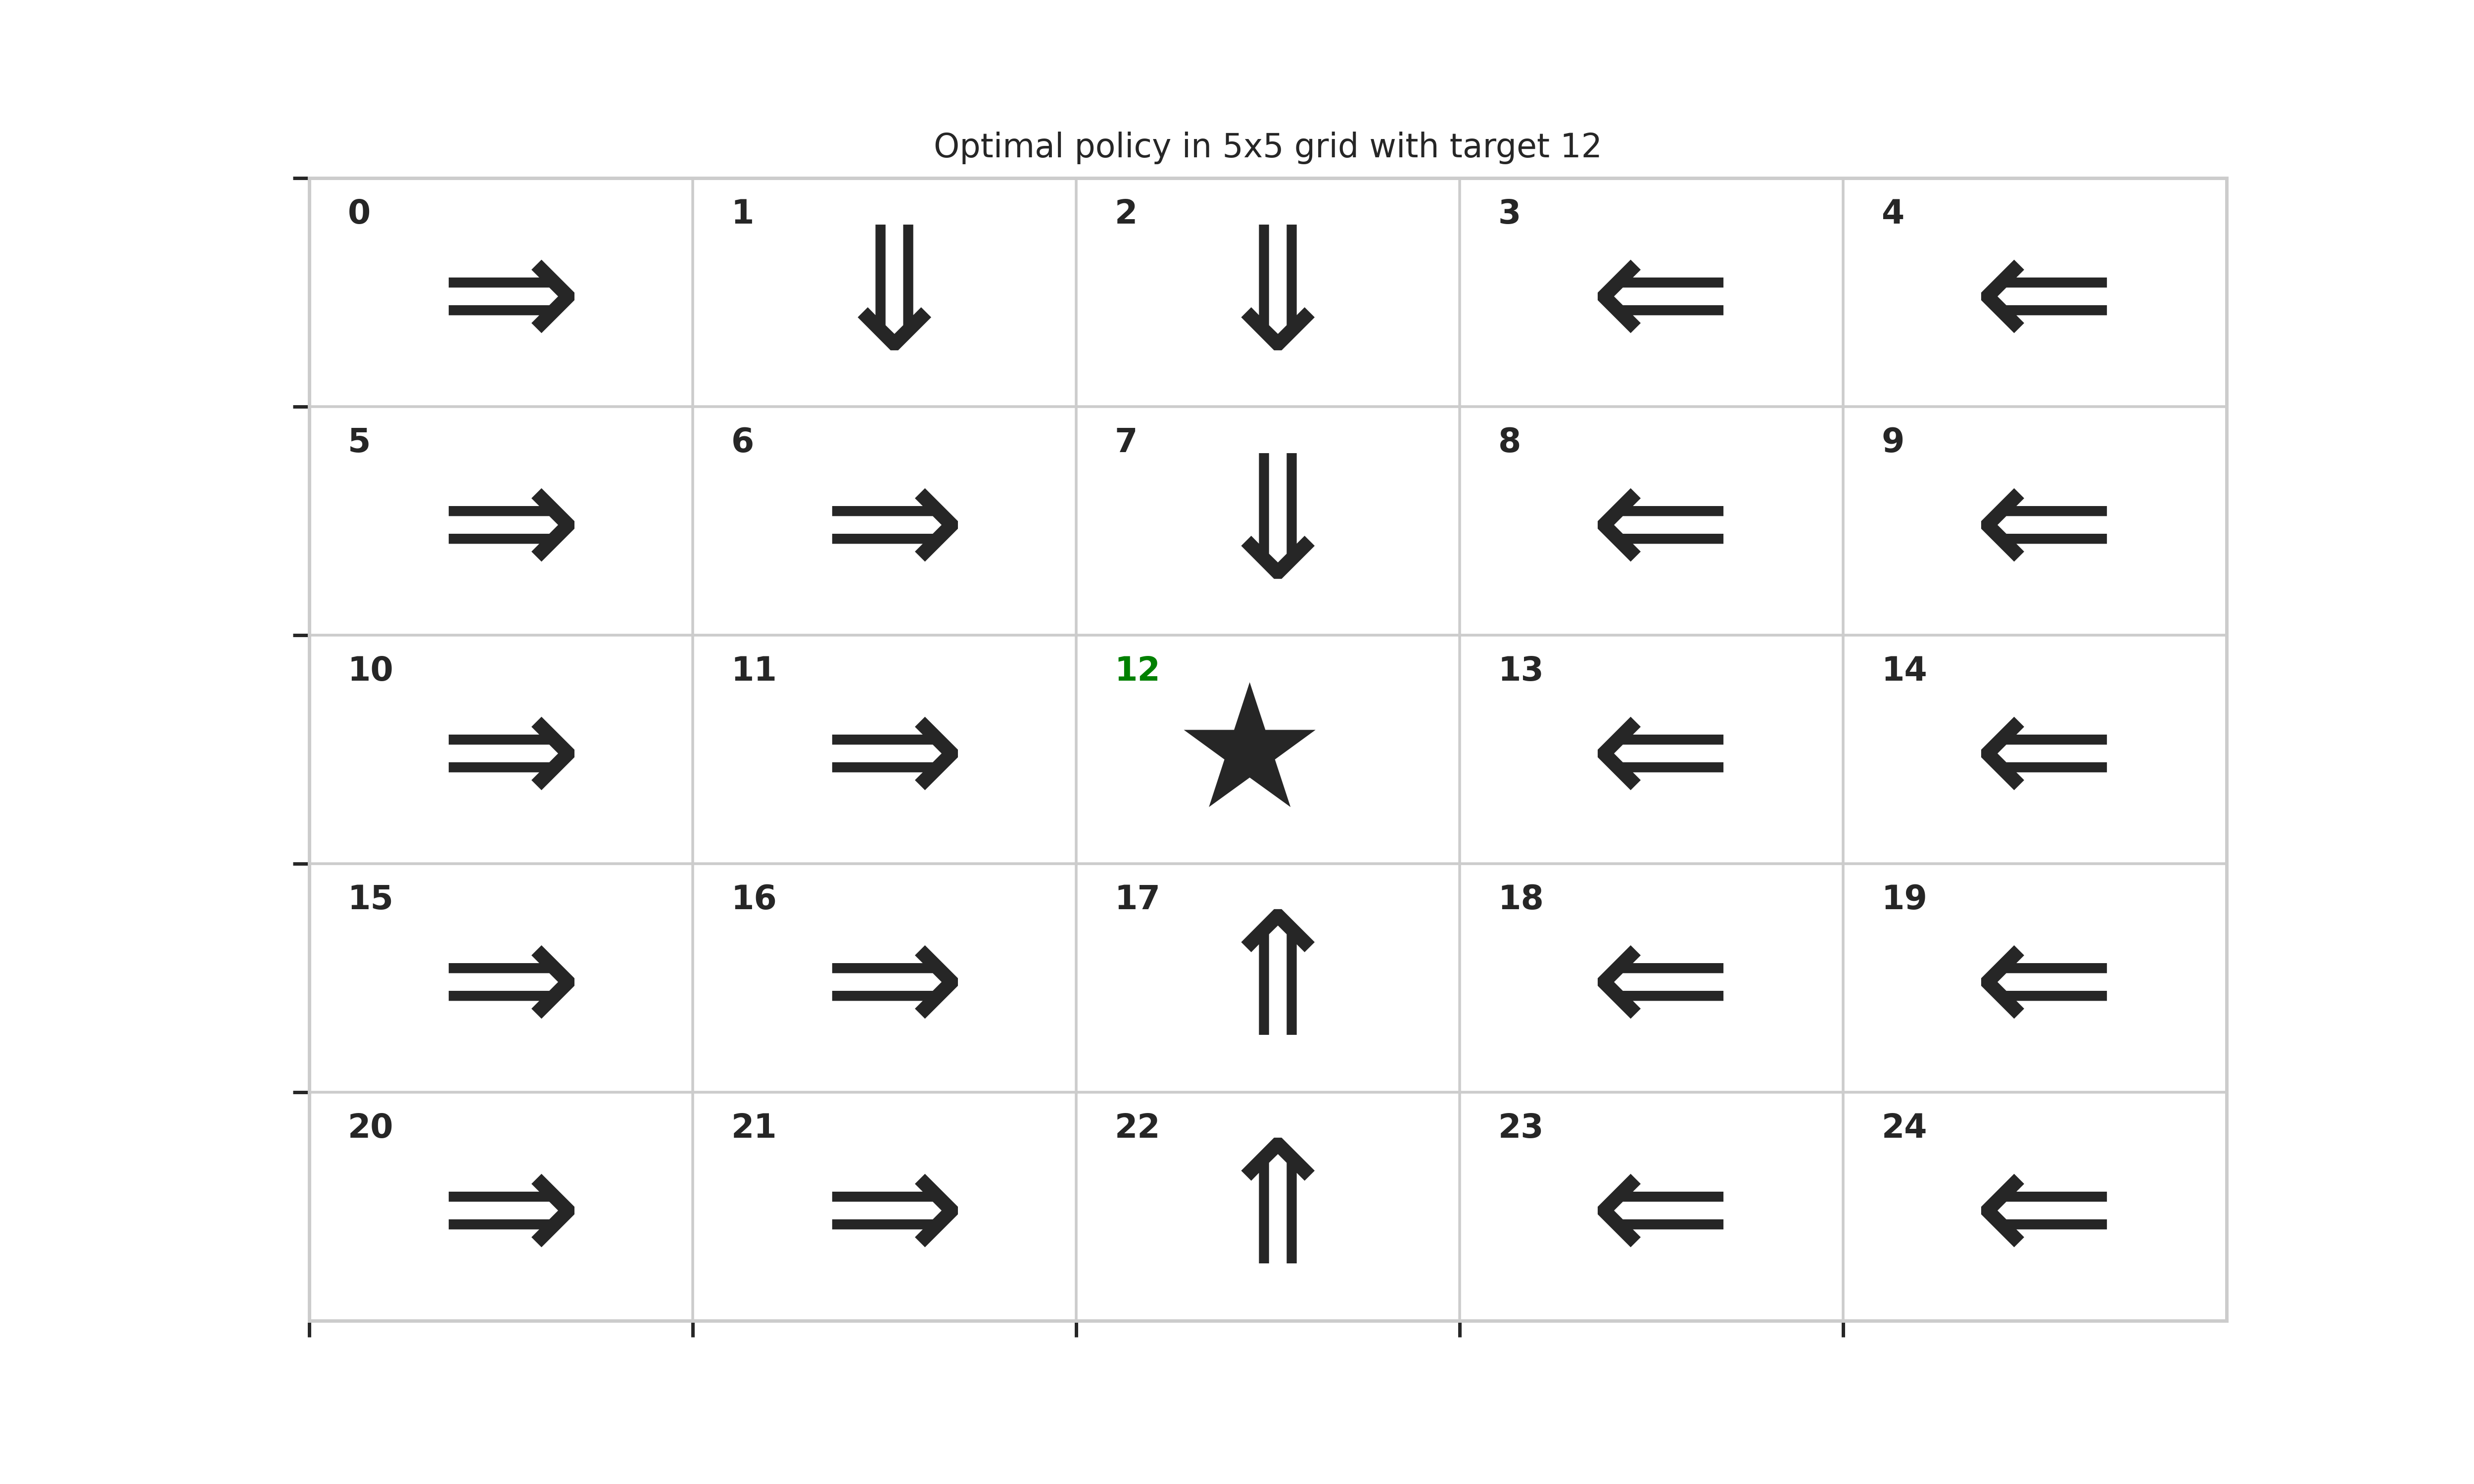
\includegraphics[width=\linewidth]{experimentation/images/Optimal policy in 5x5 grid with target 12.png}
        \caption{Optimal Policy}
    \end{subfigure}
    \begin{subfigure}[b]{0.49\linewidth}
        \centering
        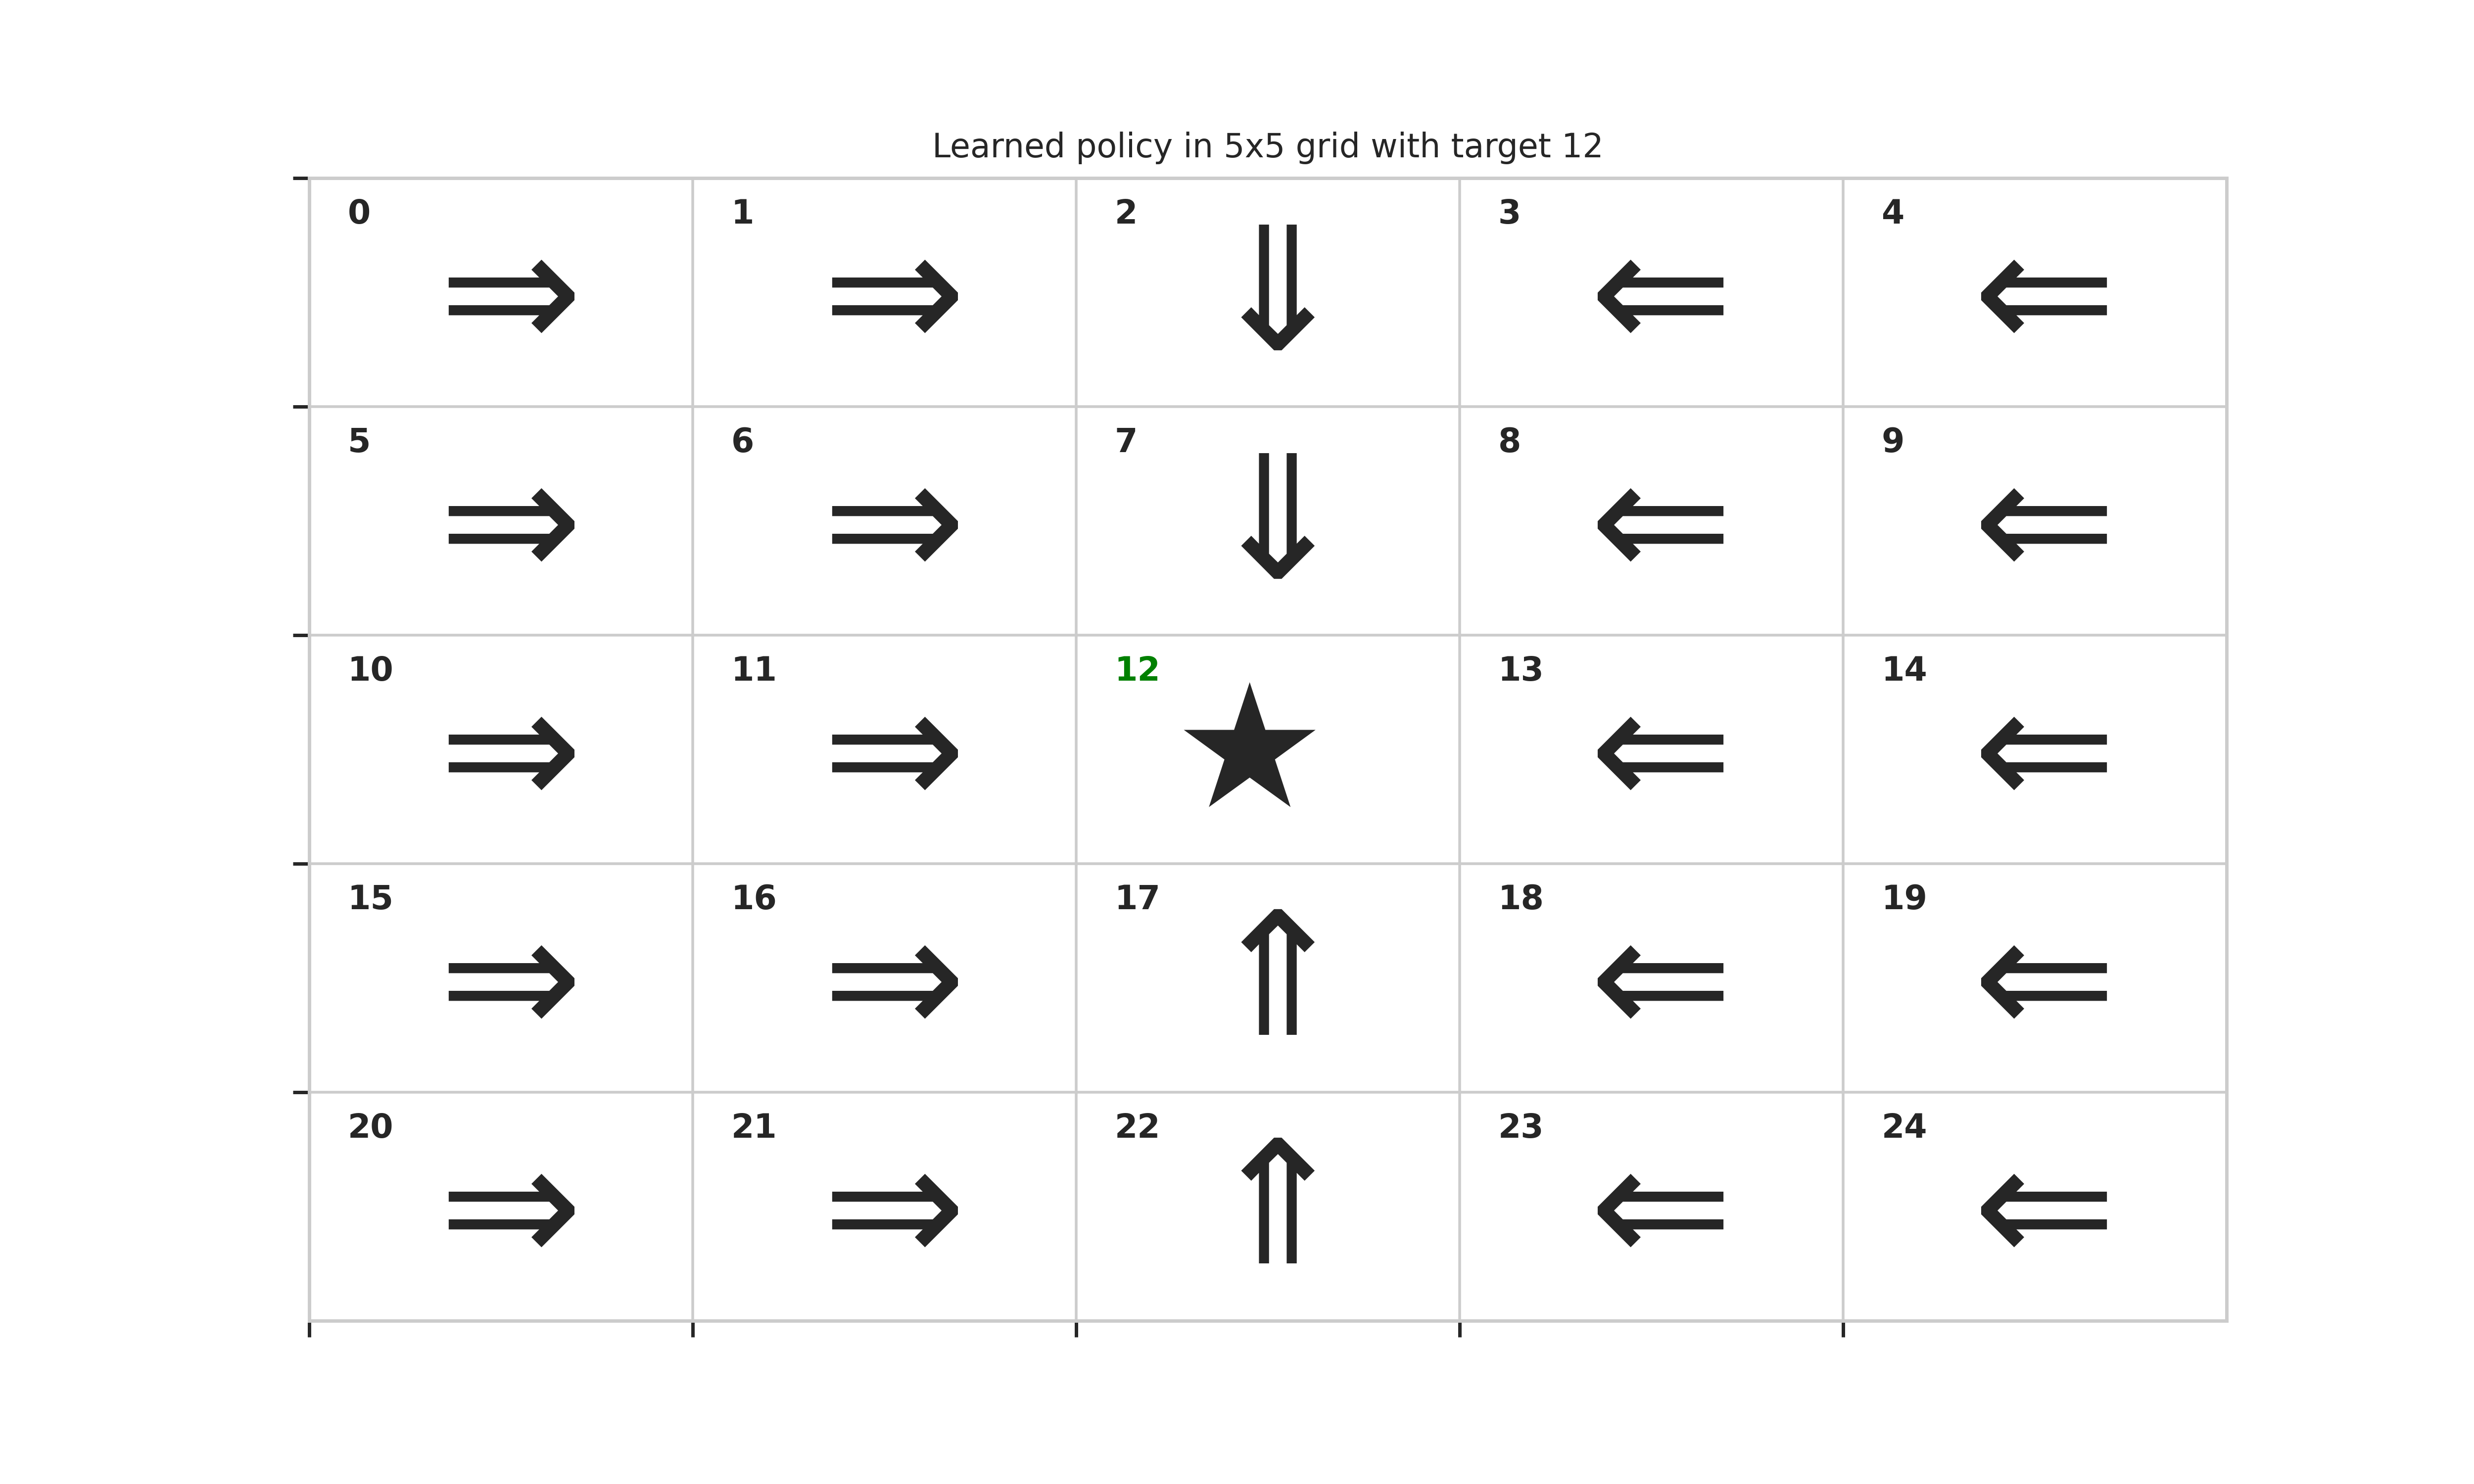
\includegraphics[width=\linewidth]{experimentation/images/Learned policy in 5x5 grid with target 12.png}
        \caption{Learned Policy}
    \end{subfigure}
    \caption{Policies for goal state set at 12.}
    \label{fig:policy_12}
\end{figure}

\begin{figure}[!htbp]
    \centering
    \begin{subfigure}[b]{0.49\linewidth}
        \centering
        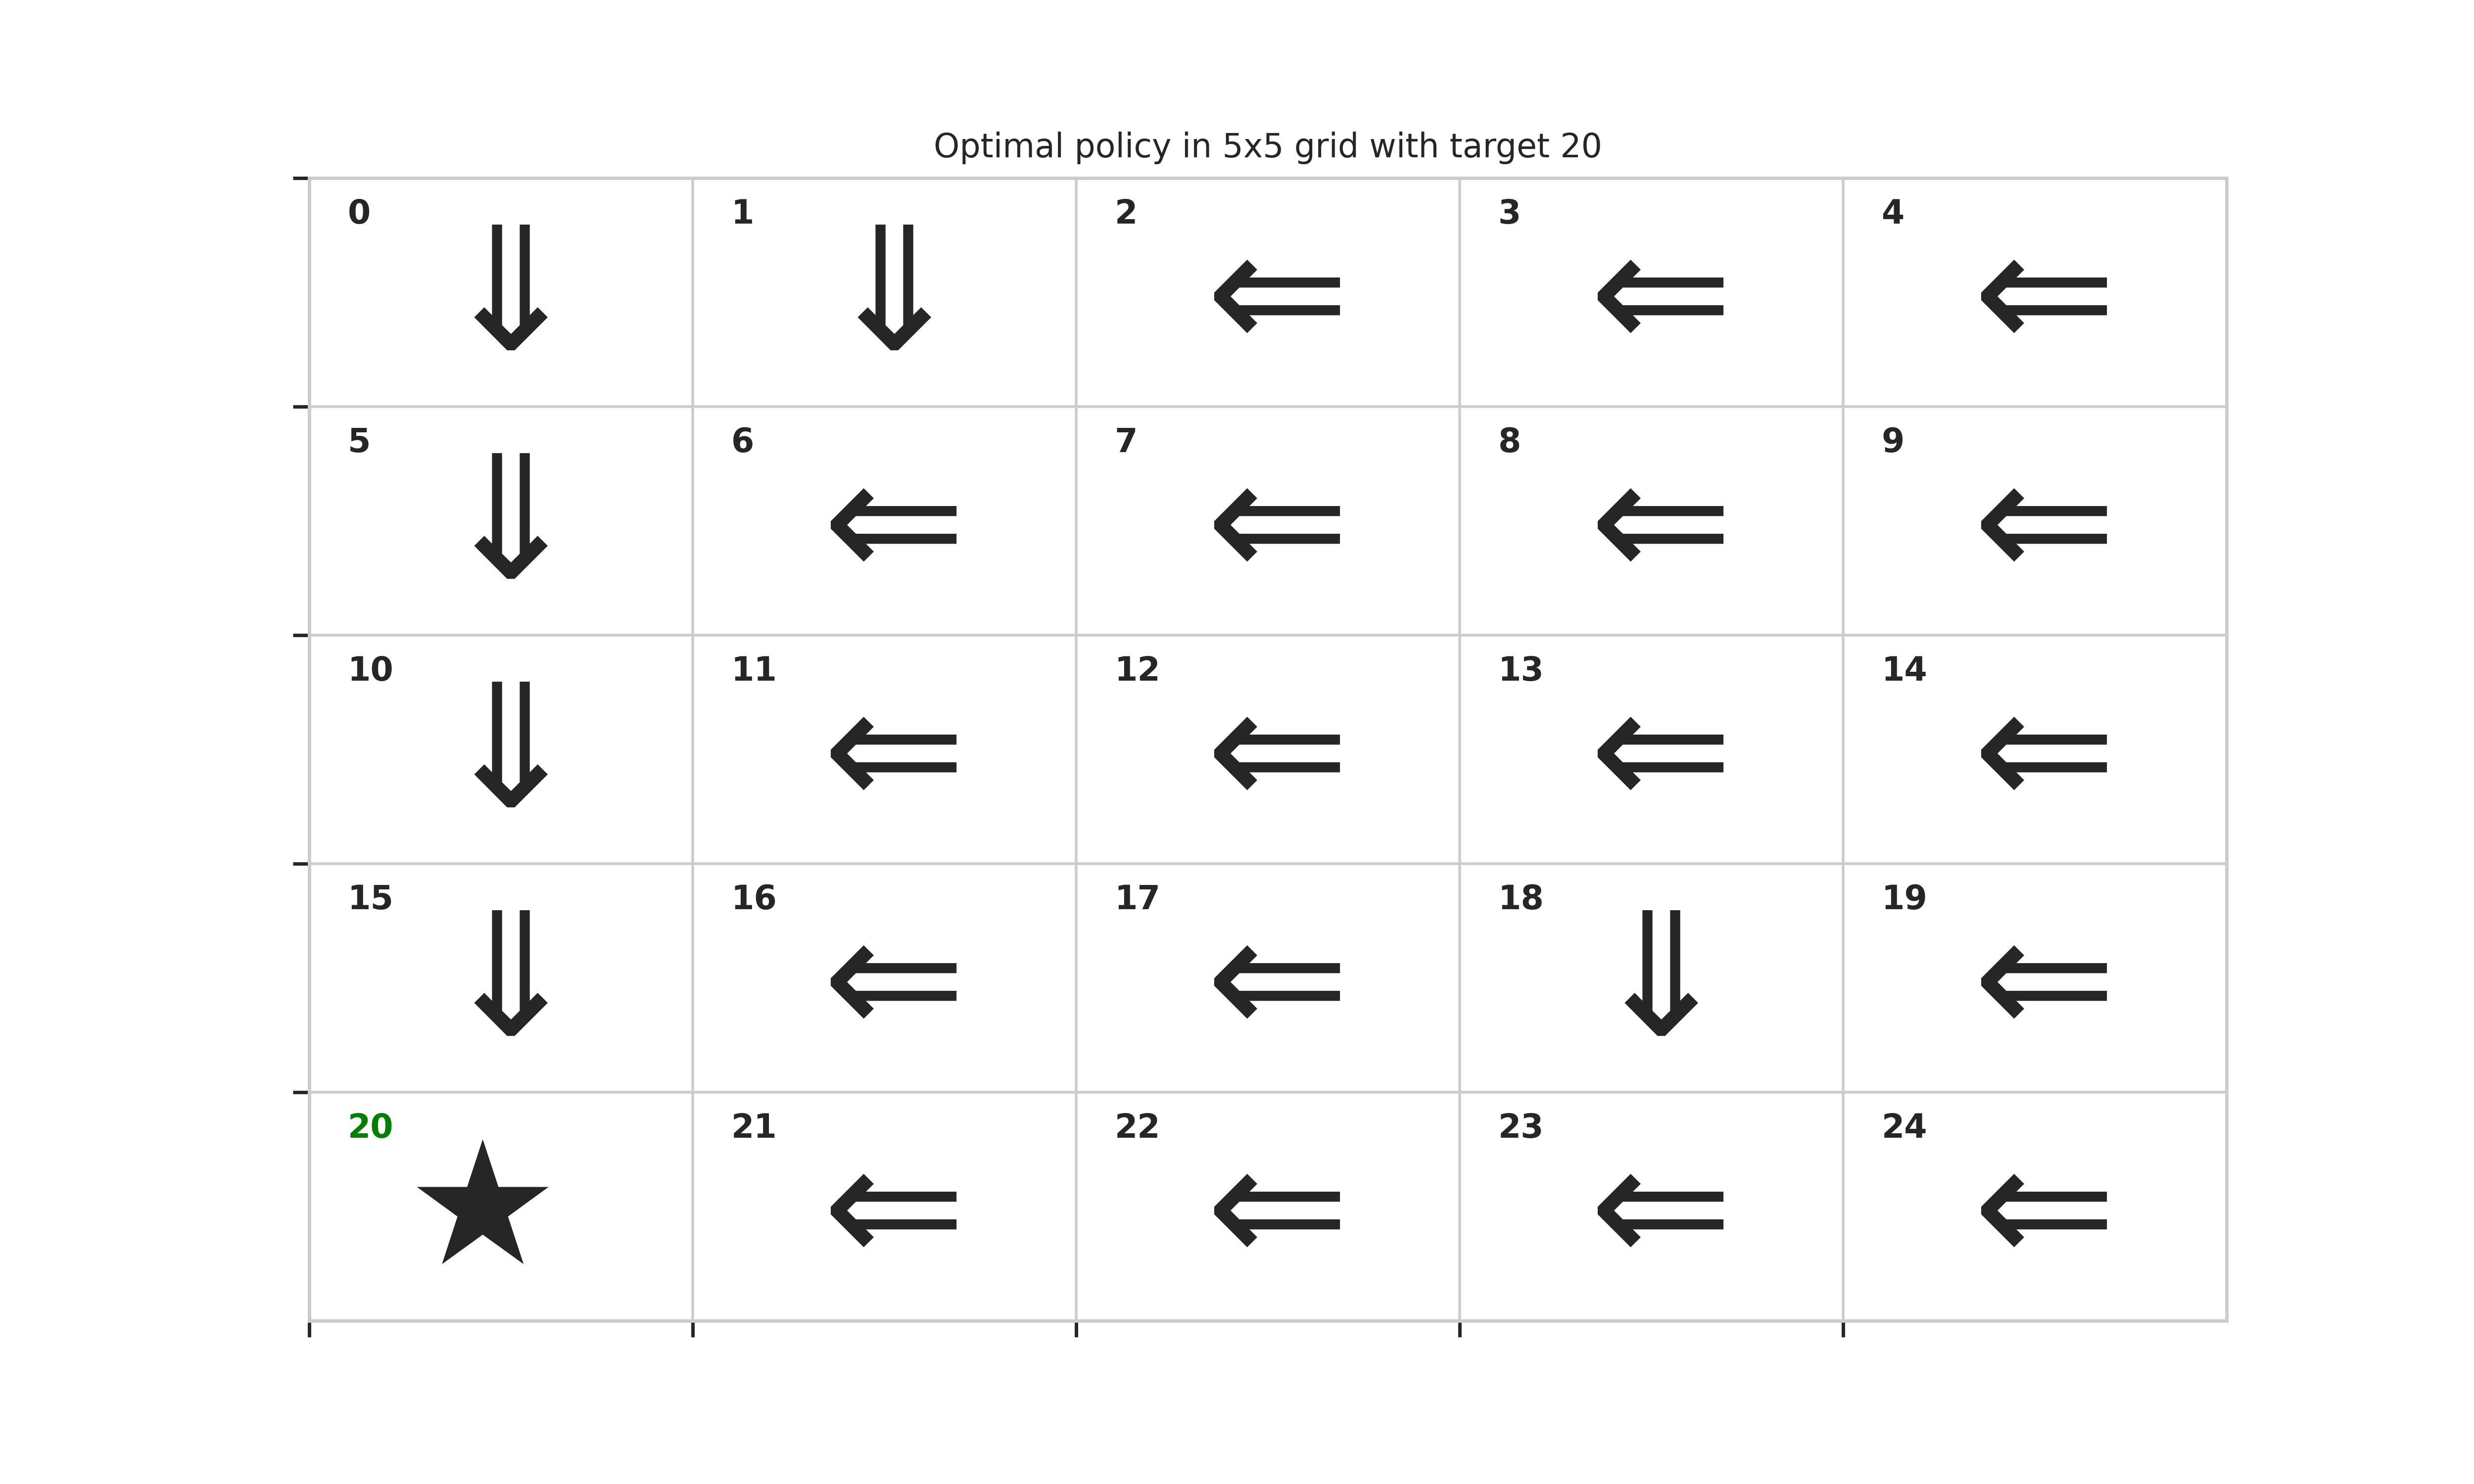
\includegraphics[width=\linewidth]{experimentation/images/Optimal policy in 5x5 grid with target 20.png}
        \caption{Optimal Policy}
    \end{subfigure}
    \begin{subfigure}[b]{0.49\linewidth}
        \centering
        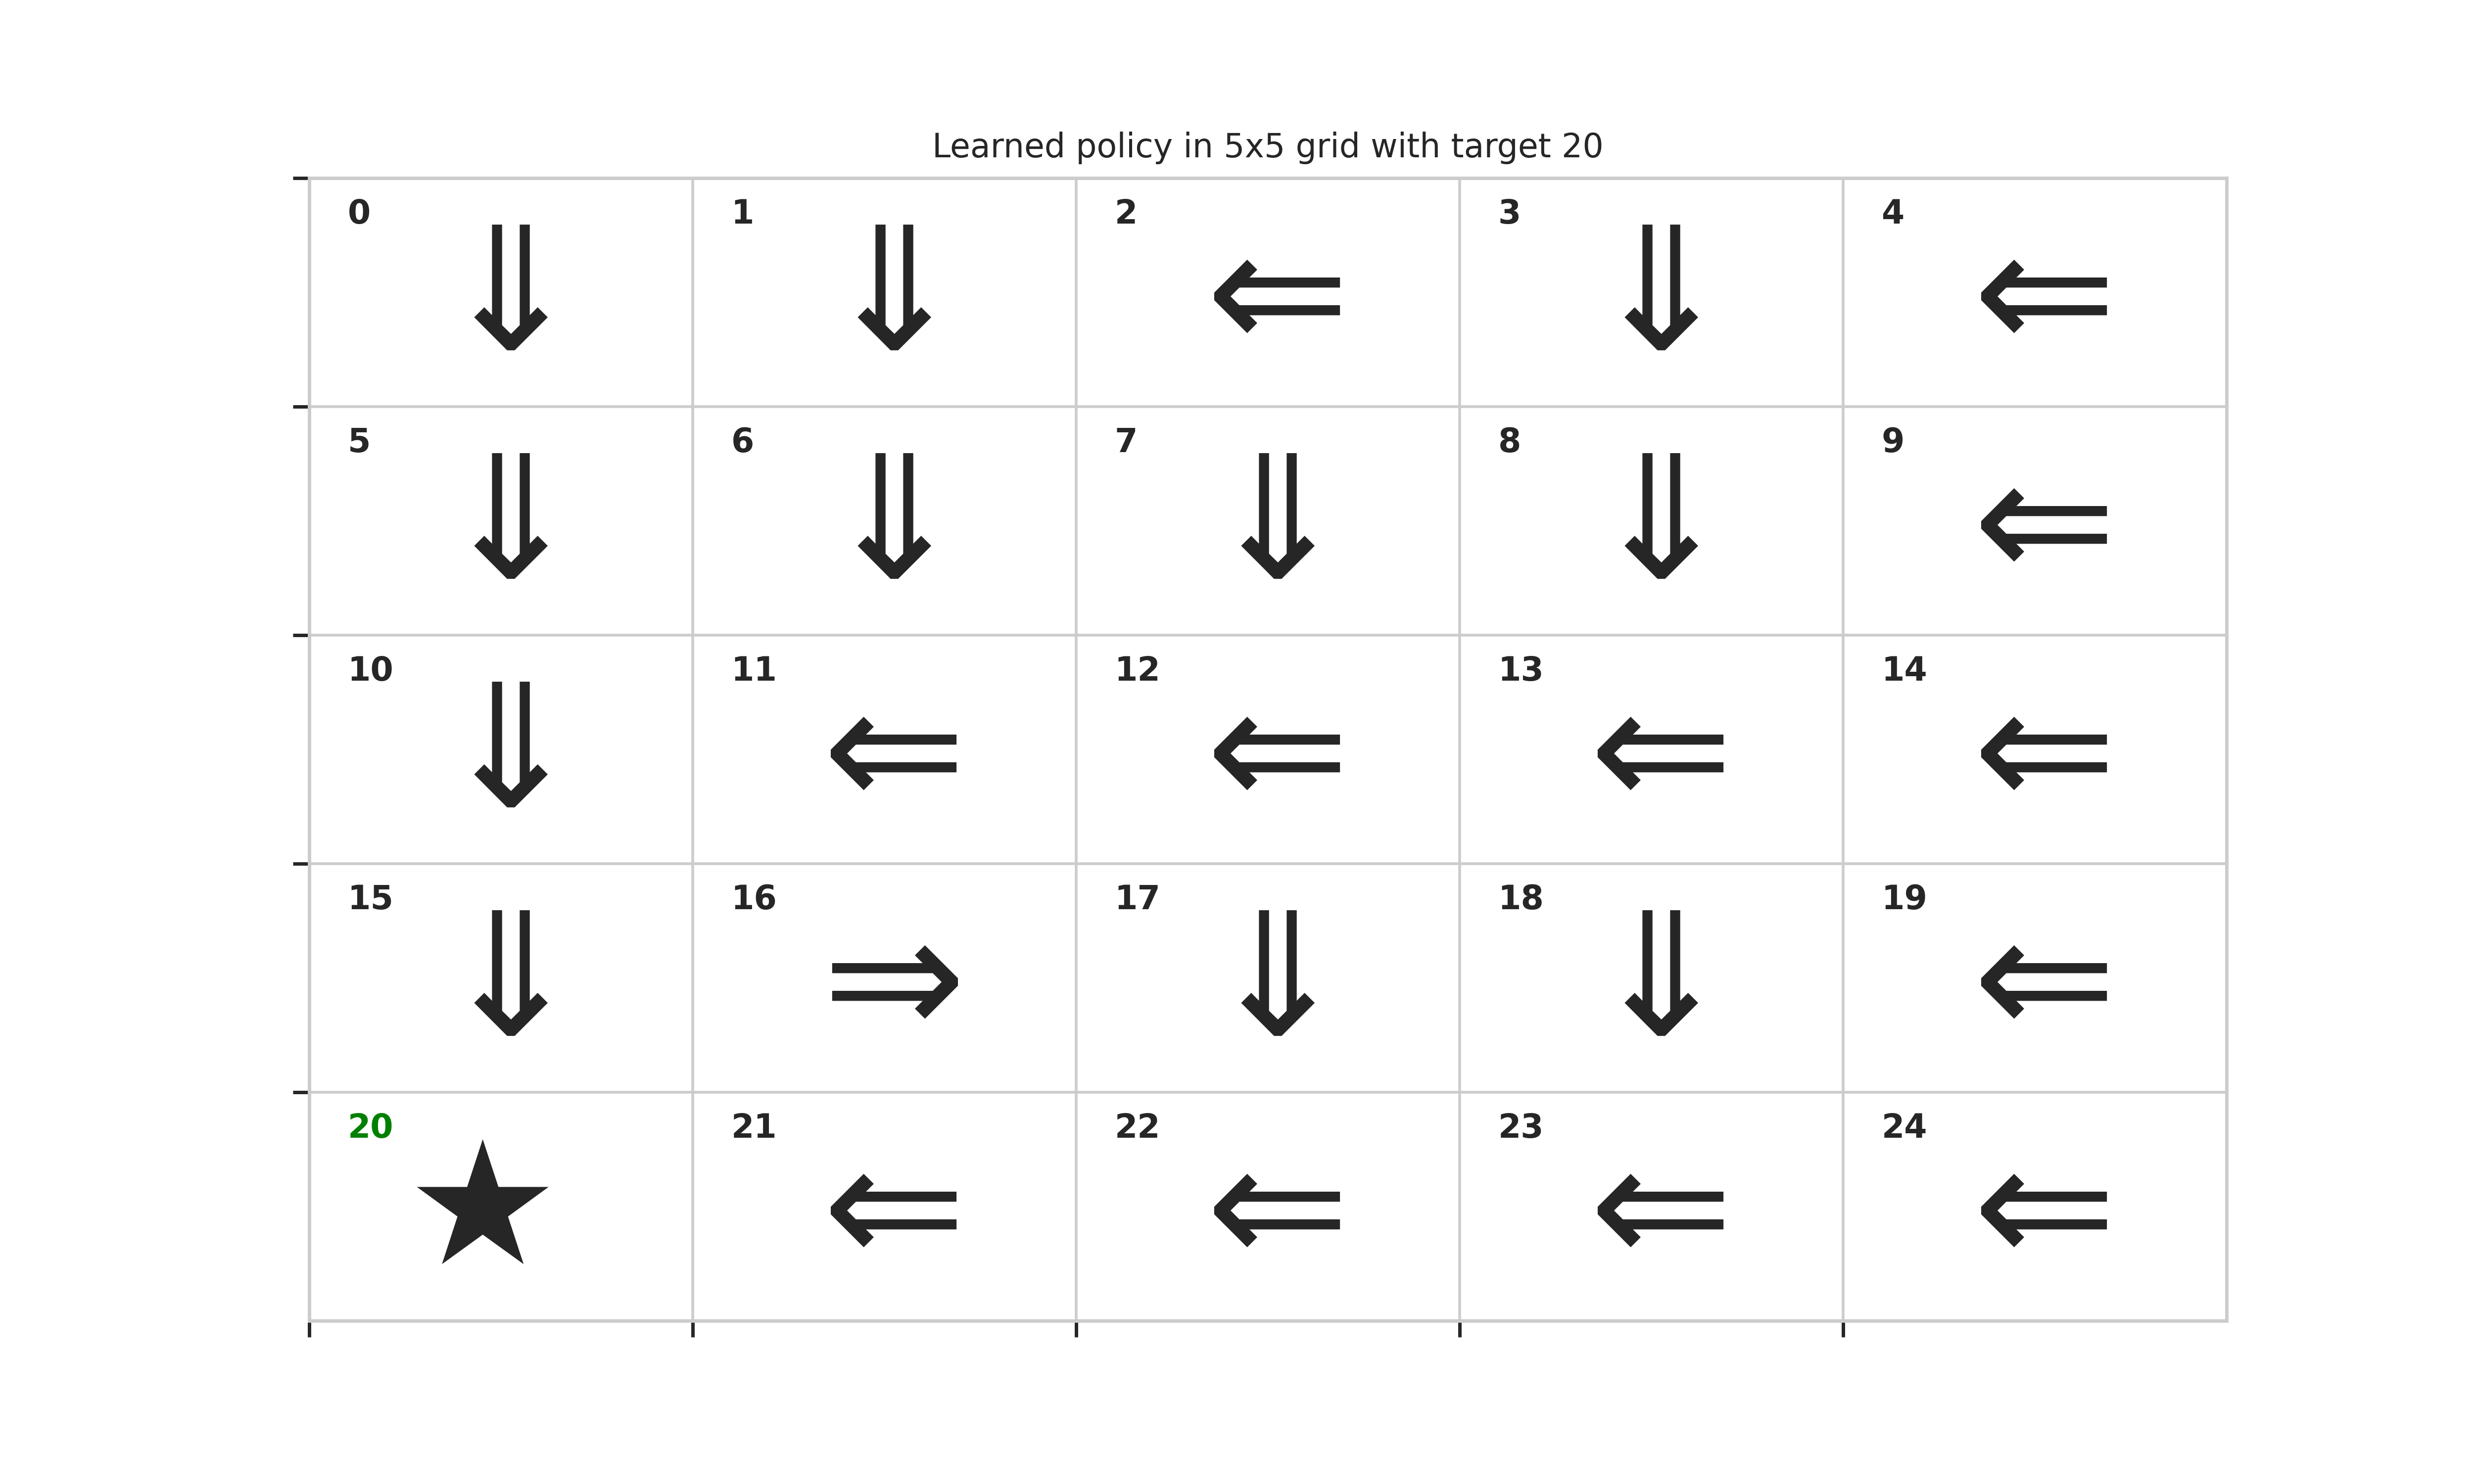
\includegraphics[width=\linewidth]{experimentation/images/Learned policy in 5x5 grid with target 20.png}
        \caption{Learned Policy}
    \end{subfigure}
    \caption{Policies for goal state set at 20.}
    \label{fig:policy_20}
\end{figure}

\newpage
